%%%%%%%% ICML 2021 EXAMPLE LATEX SUBMISSION FILE %%%%%%%%%%%%%%%%%

\documentclass{article}

% Recommended, but optional, packages for figures and better typesetting:
\usepackage{microtype}
\usepackage{graphicx}
%\usepackage{subfigure}
\usepackage{booktabs} % for professional tables
\usepackage{amsfonts}
\usepackage{multirow}
\usepackage{amsmath}
\usepackage{caption}
\usepackage{subcaption}
\usepackage{natbib}
%\usepackage[T1]{fontenc}

% hyperref makes hyperlinks in the resulting PDF.
% If your build breaks (sometimes temporarily if a hyperlink spans a page)
% please comment out the following usepackage line and replace
% \usepackage{icml2021} with \usepackage[nohyperref]{icml2021} above.
\usepackage{hyperref}

% Attempt to make hyperref and algorithmic work together better:
\newcommand{\theHalgorithm}{\arabic{algorithm}}

% Use the following line for the initial blind version submitted for review:
%\usepackage{icml2021}

% If accepted, instead use the following line for the camera-ready submission:
\usepackage[accepted]{icml2021}

% The \icmltitle you define below is probably too long as a header.
% Therefore, a short form for the running title is supplied here:
\icmltitlerunning{TDHNN: Time-Dependent Hamiltonian Neural Networks}

\bibliographystyle{icml2021}
\begin{document}

\section*{Appendix}

\subsection*{A.1}

Why can we not including damping into the Hamiltonian? Let us take the following damped system:
\begin{equation}
\ddot{\mathbf{q}} = -\mathbf{q} - \delta\dot{\mathbf{q}}
\end{equation}
where we know $\mathbf{p}=m\dot{\mathbf{q}}$ which implies $\dot{\mathbf{q}} = m^{-1}\mathbf{p}$.

Then, the integral of the right hand side with respect to q will give us:

\begin{equation}
\frac{\mathbf{q}^2}{2} + \delta \mathbf{q} \dot{\mathbf{q}}
\end{equation}

The equation above looks like a modified potential function which can be combined with a kinetic energy term to give a Hamiltonian s.t.:

\begin{equation}
\mathcal{H} =\frac{ \mathbf{p}^2}{2m} + \frac{\mathbf{q}^2}{2} + \delta \mathbf{q} \dot{\mathbf{q}}
\end{equation}

However, although we can recover the differential equation for $\ddot{\mathbf{q}}$ by $-\frac{\partial\mathcal{H}}{\mathrm{d}\mathbf{q}}  =-\mathbf{q} - \delta\dot{\mathbf{q}} = \ddot{\mathbf{q}}$, we violate the rule that $\dot{\mathbf{q}} = m^{-1}\mathbf{p}$ since $ \frac{\partial\mathcal{H}}{\mathrm{d}\mathbf{p}} =  \dot{\mathbf{q}} +\delta \mathbf{q} \neq \dot{\mathbf{q}} $.

Indeed an alternative formulation that uses exponentiated time can allow us to represent a Hamiltonian for the damped system but this is not within the scope of our study as the formalism does not explain how to include external forcing.

%\begin{table*}[ht!]
%\caption{Test Rollout MSE} 
%\centering % centering table
%\resizebox{\textwidth}{!}{\begin{tabular}{c  cc cc cc cc cc} % creating eight columns
%\hline\hline %inserting double-line
%\multirow{2}{*}{Method}&\multicolumn{2}{c}{Ideal Mass Spring}&\multicolumn{2}{c}{Damped Mass Spring} & \multicolumn{2}{c}{Forced Mass Spring (1)} &\multicolumn{2}{c}{Forced Mass Spring (2)} & \multicolumn{2}{c}{Duffing Non-Chaotic} \\
%\cline{2-11} % inserts single-line
% & State & Energy & State & Energy & State & Energy & State & Energy & State & Energy \\
%\hline
%Baseline NN &\\ % Entering row contents
%HNN &\\
%TDHNN &\\
%TDHNN4 &
%\\% [1ex] adds vertical space
%\hline % inserts single-line
%\end{tabular}}
%\label{tab:tests}
%\end{table*}

\pagebreak
\twocolumn
\subsection*{B}

\begin{figure}[!htb]
\centering
\captionsetup{justification=centering}
\begin{subfigure}[b]{0.48\textwidth}
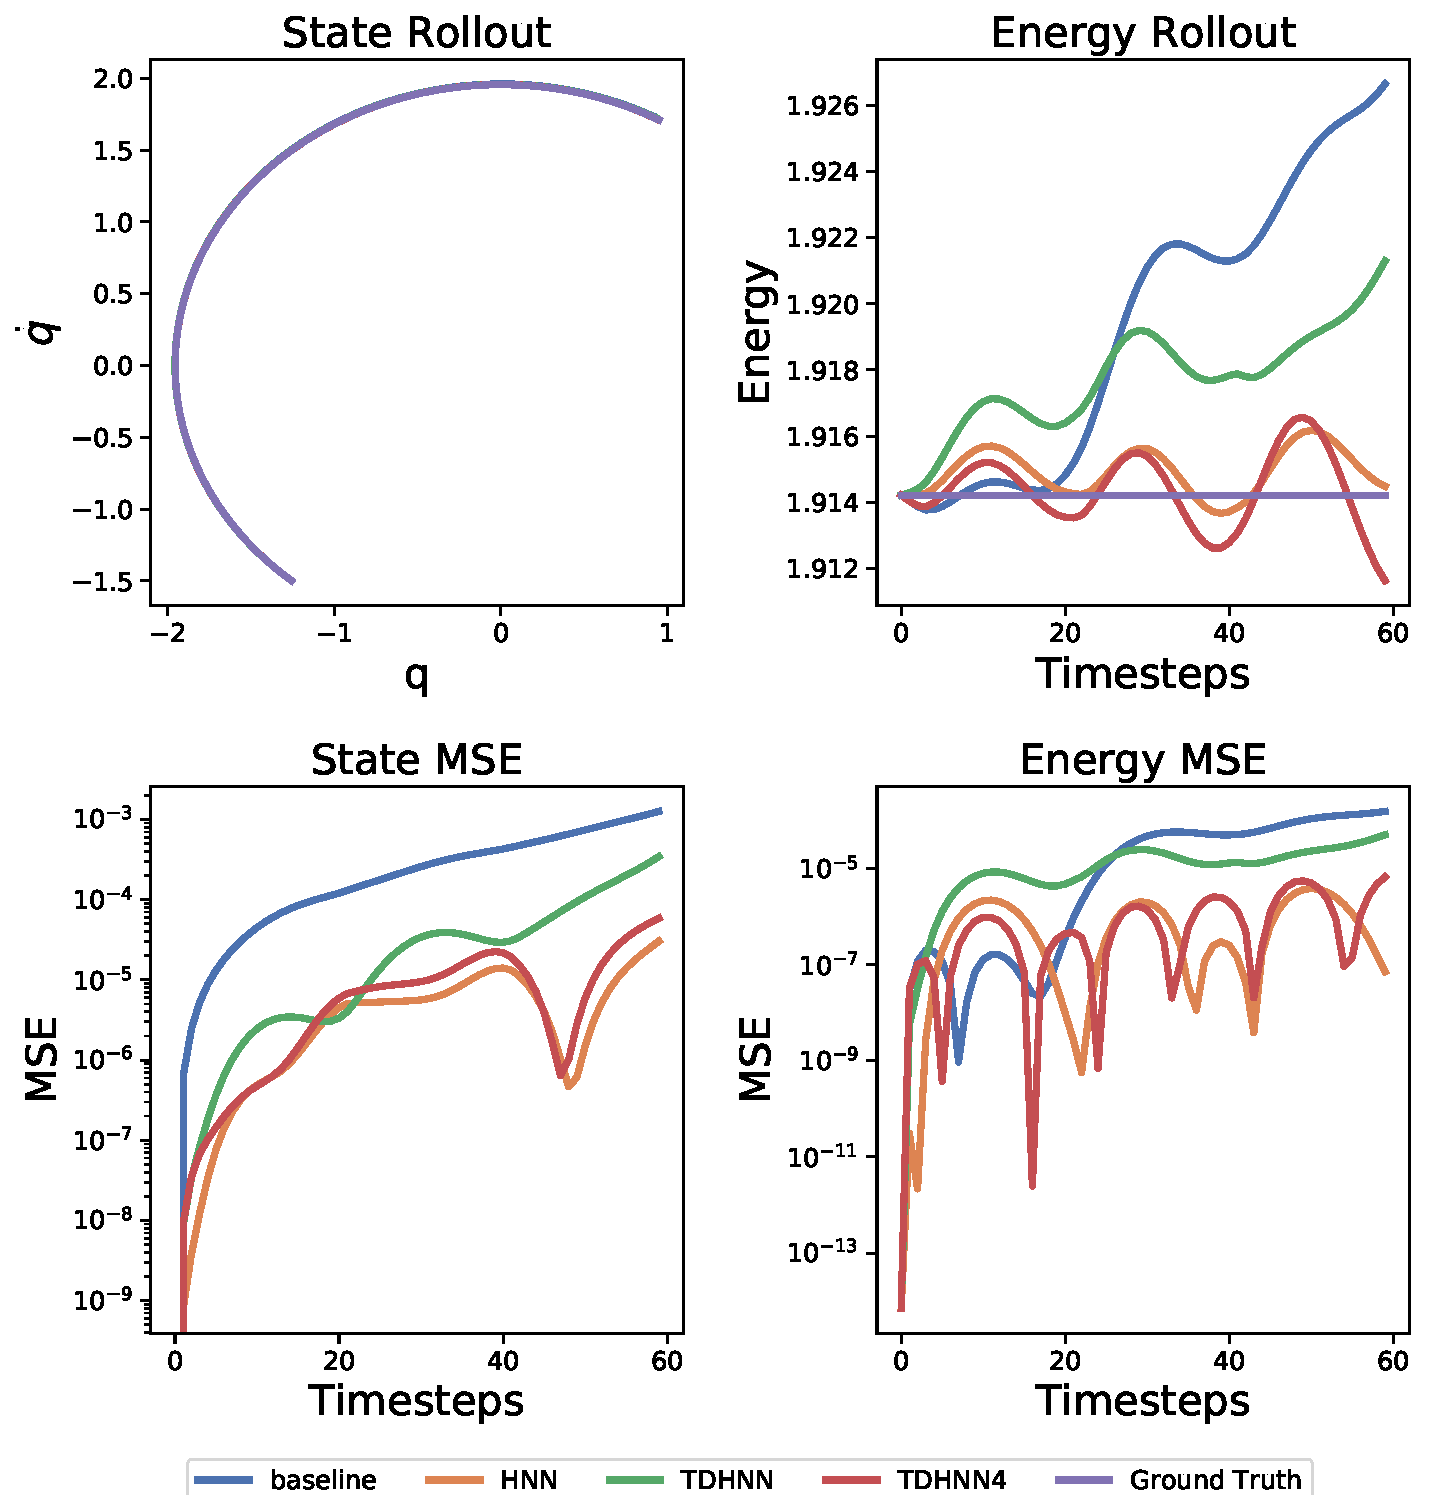
\includegraphics[width=\textwidth]{figures/figures/mass_spring/1/mass_spring_long_0.pdf}
\caption{State and energy rollout of an initial condition from the test set}
\end{subfigure}
\begin{subfigure}[b]{0.48\textwidth}
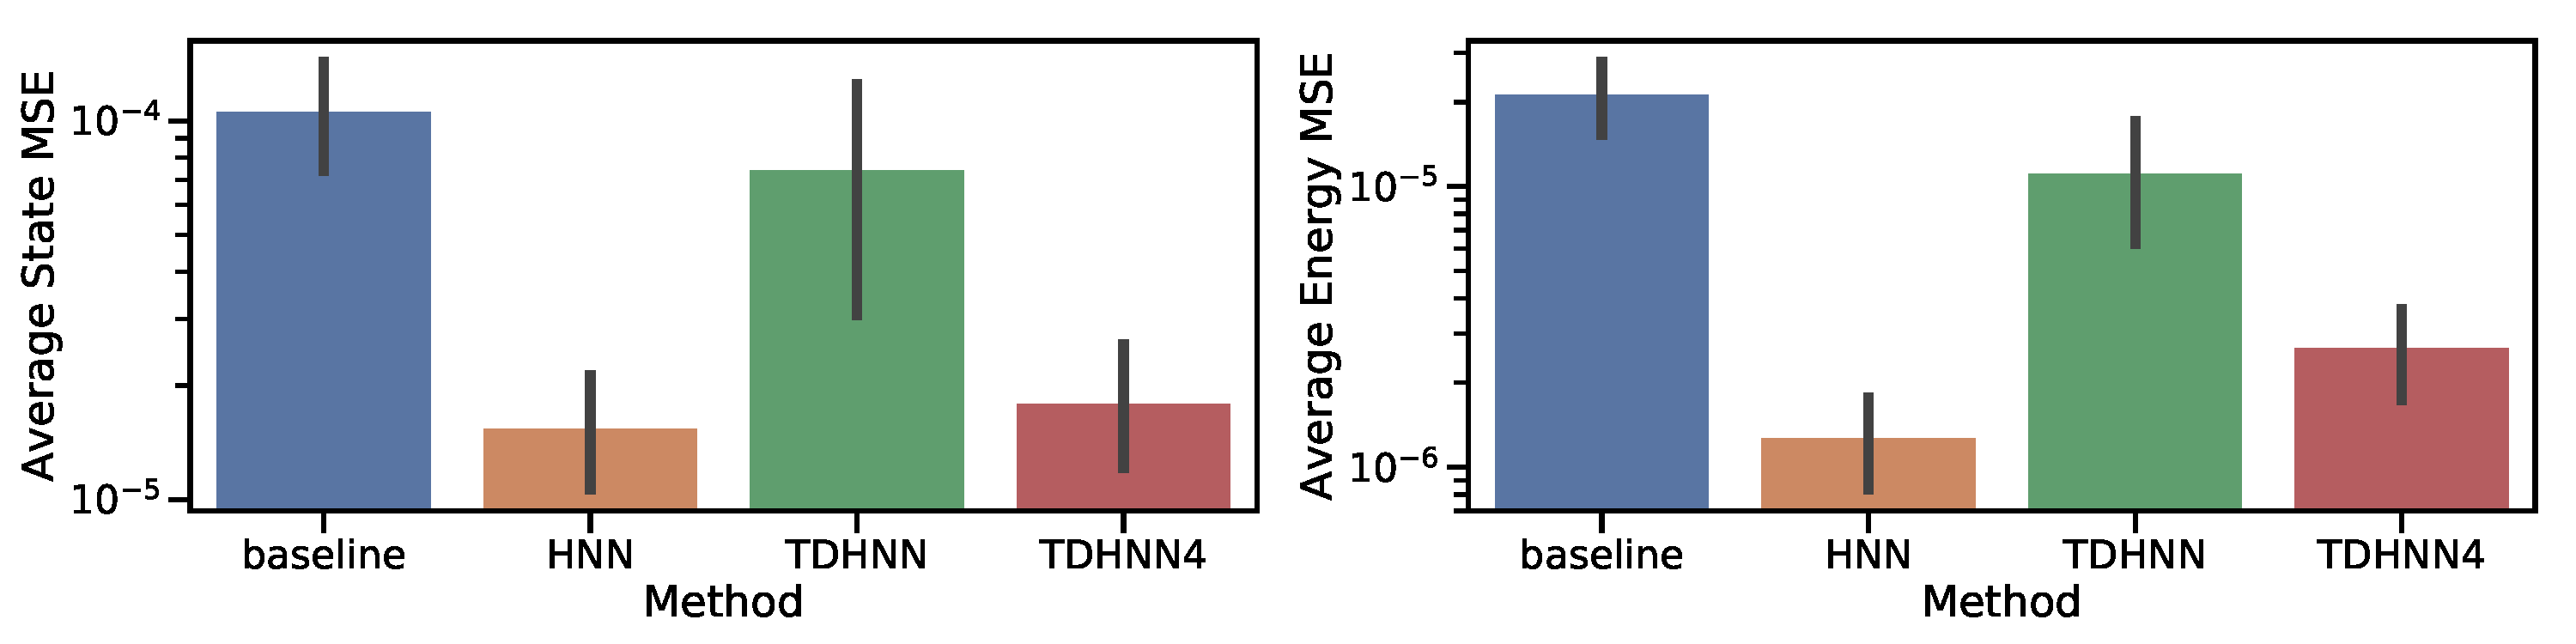
\includegraphics[width=\textwidth]{figures/figures/mass_spring/1/mass_spring_errors_0.pdf}
\caption{The average state and energy MSE across 25 test points}
\end{subfigure}
\begin{subfigure}[b]{0.48\textwidth}
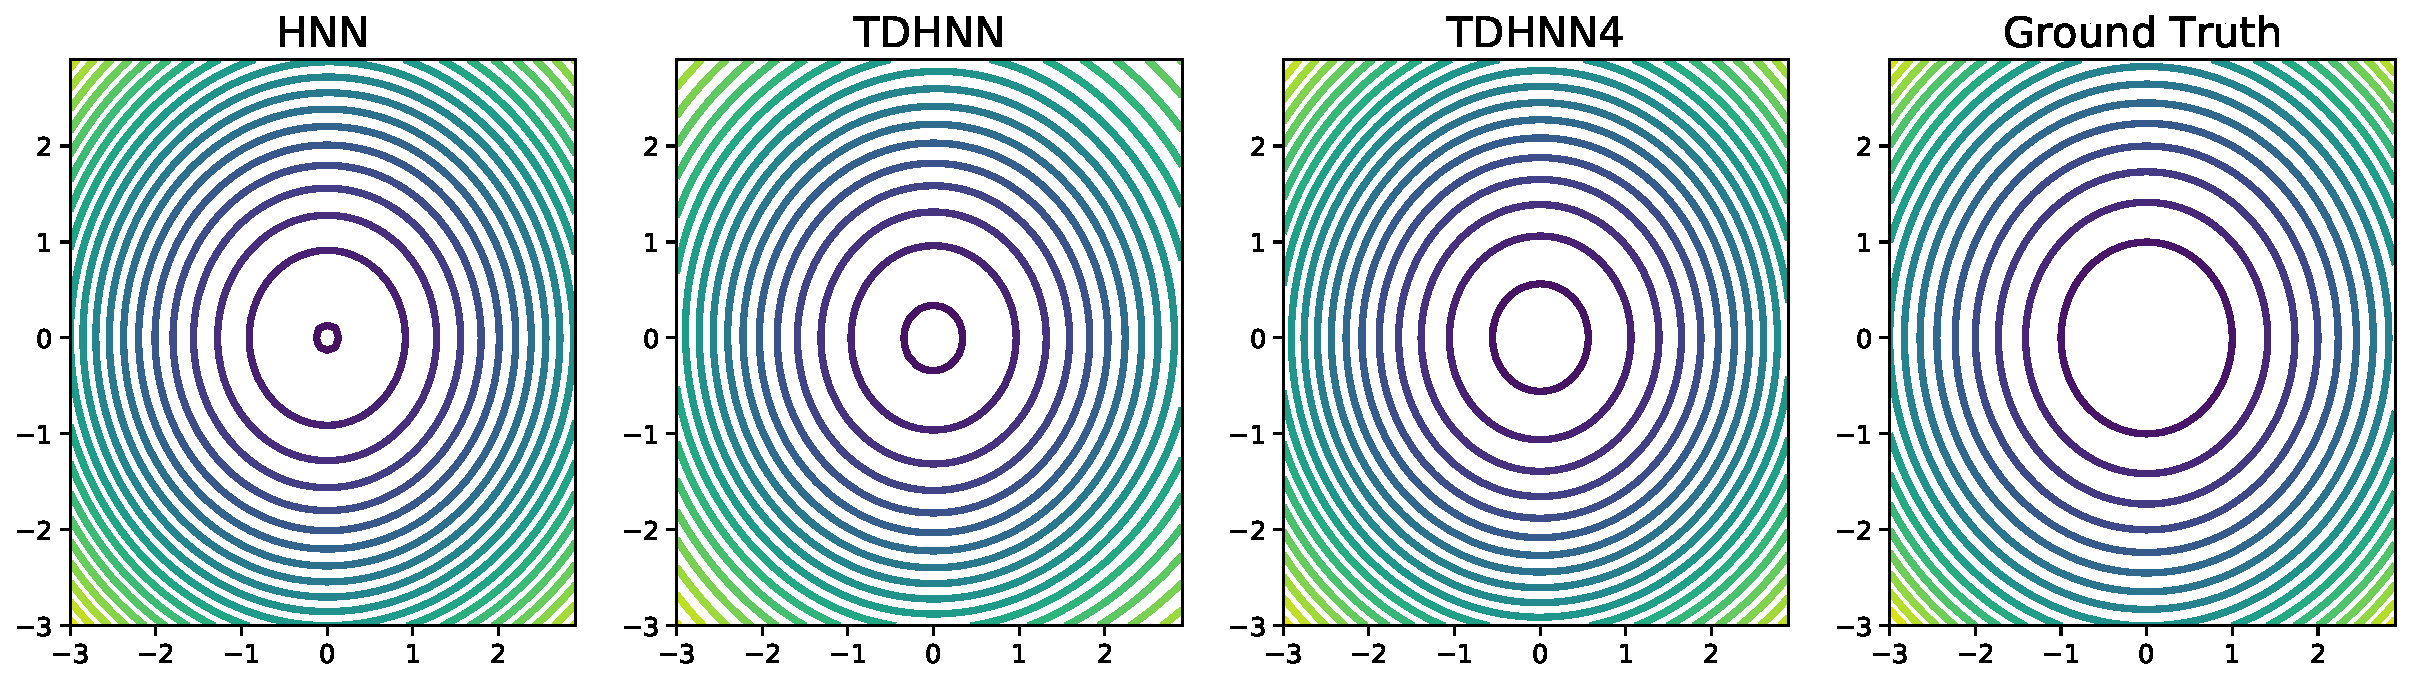
\includegraphics[width=\textwidth]{figures/figures/mass_spring/1/mass_spring_hamiltonian_0.pdf}
\caption{The learnt Hamiltonian across methods}
\end{subfigure}
\begin{subfigure}[b]{0.48\textwidth}
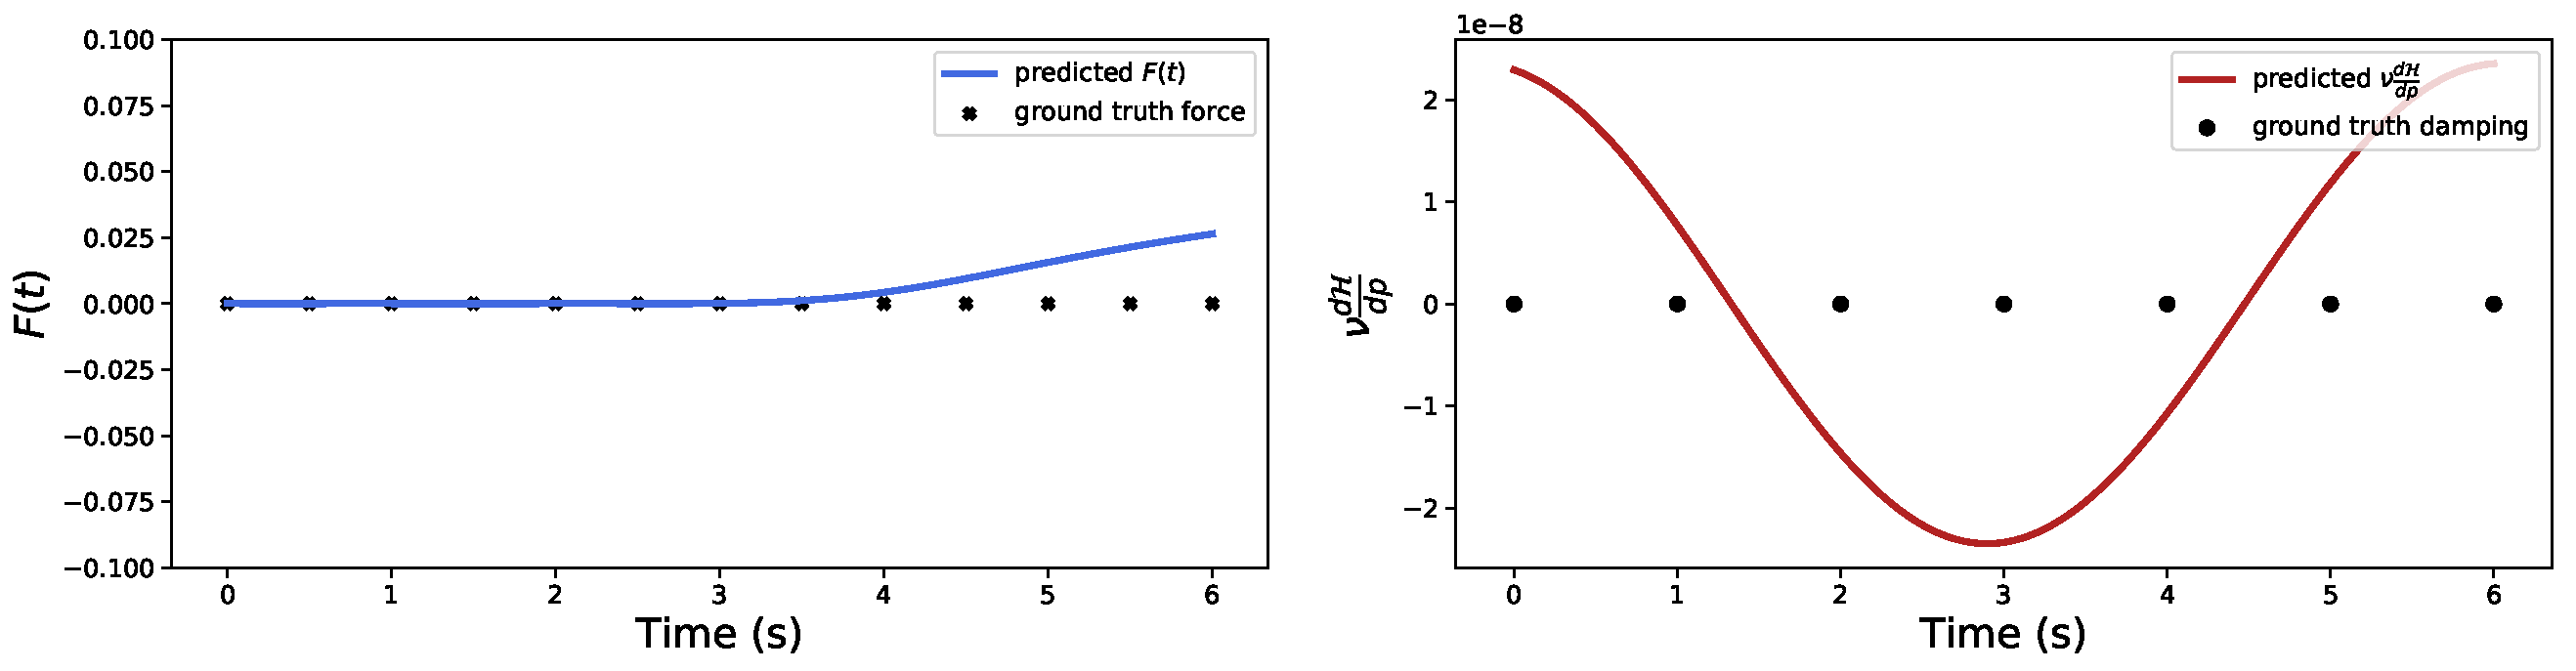
\includegraphics[width=\textwidth]{figures/figures/mass_spring/1/mass_spring_dpdt_new_0.pdf}
\caption{The learnt force and damping of TDHNN4}
\end{subfigure}
\label{mspring_full}
\end{figure}
\begin{figure}[!htb]
\centering
\captionsetup{justification=centering}
\begin{subfigure}[b]{0.48\textwidth}
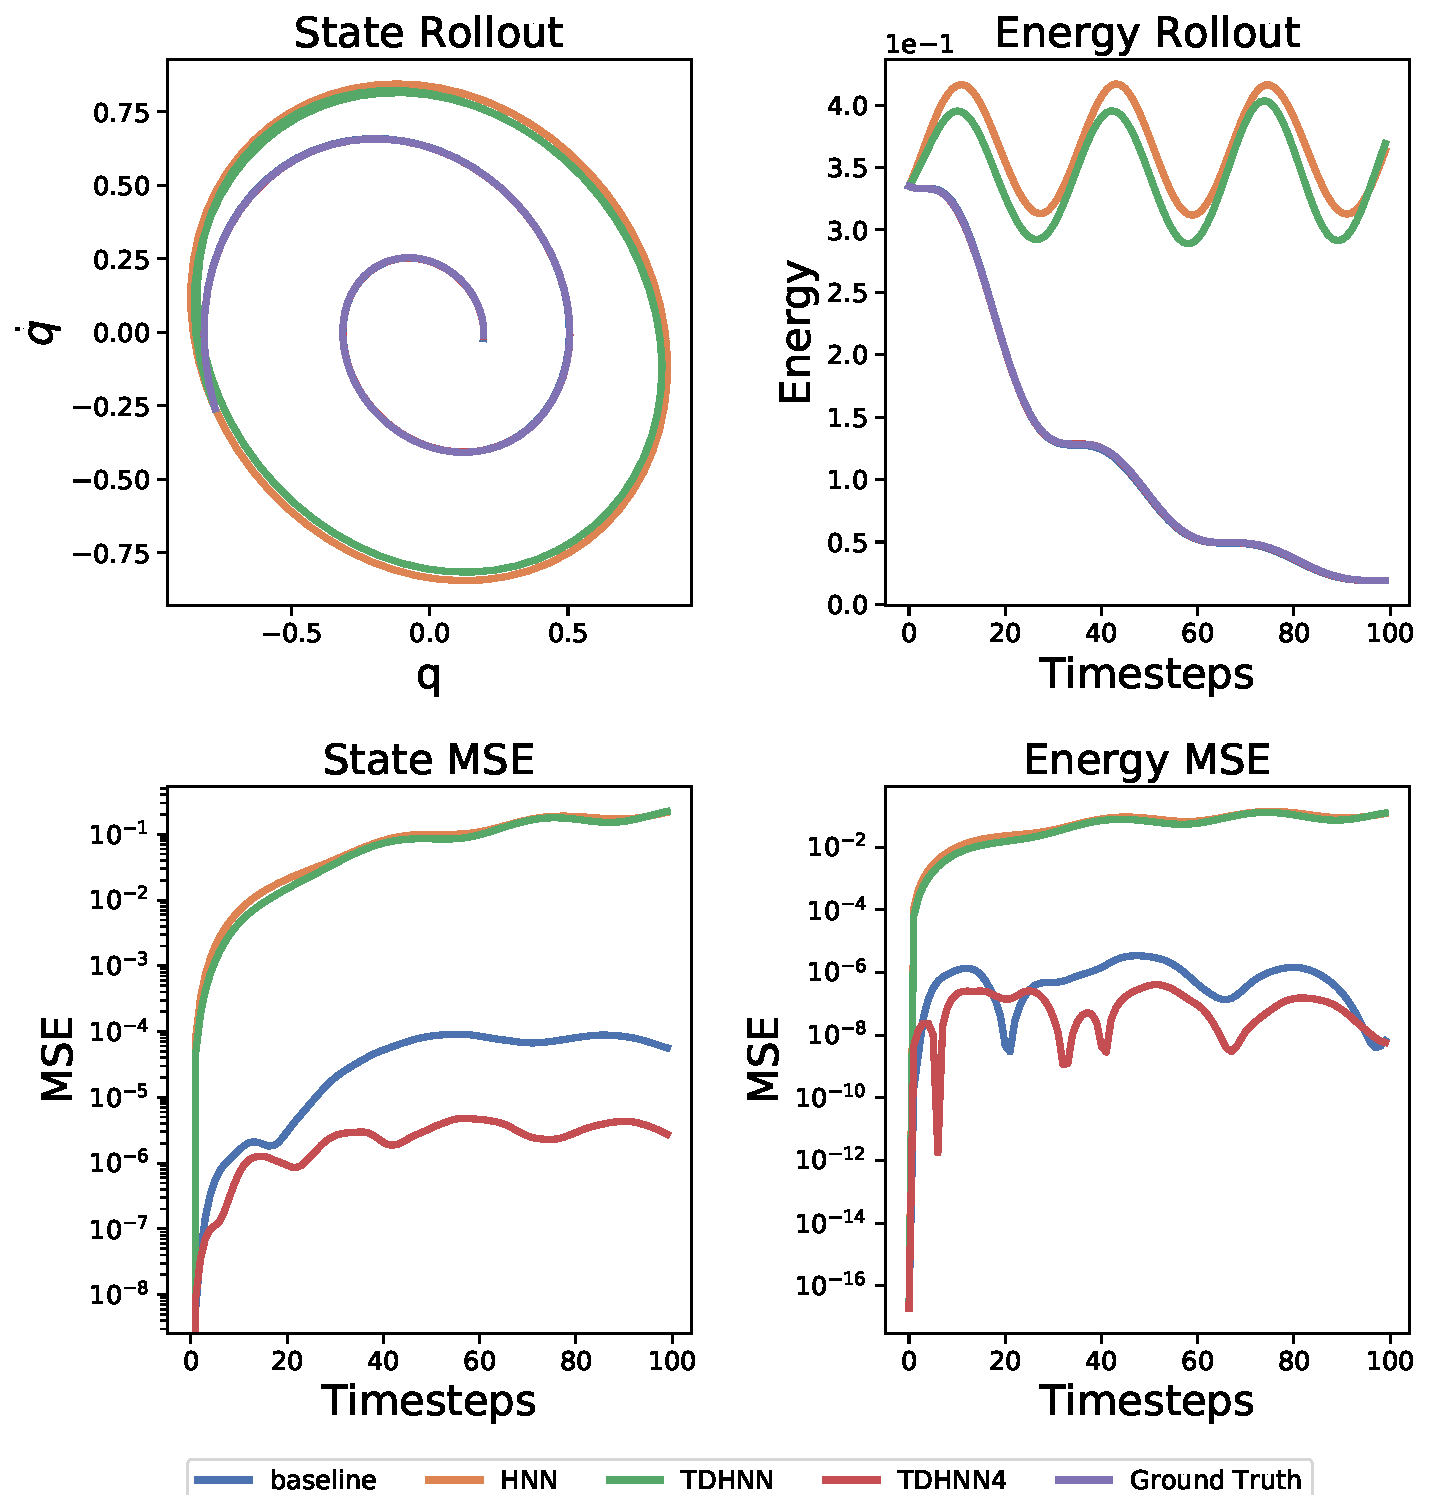
\includegraphics[width=\textwidth]{figures/figures/damped/1/damped_long_0.pdf}
\caption{State and energy rollout of an initial condition from the test set}
\end{subfigure}
\begin{subfigure}[b]{0.48\textwidth}
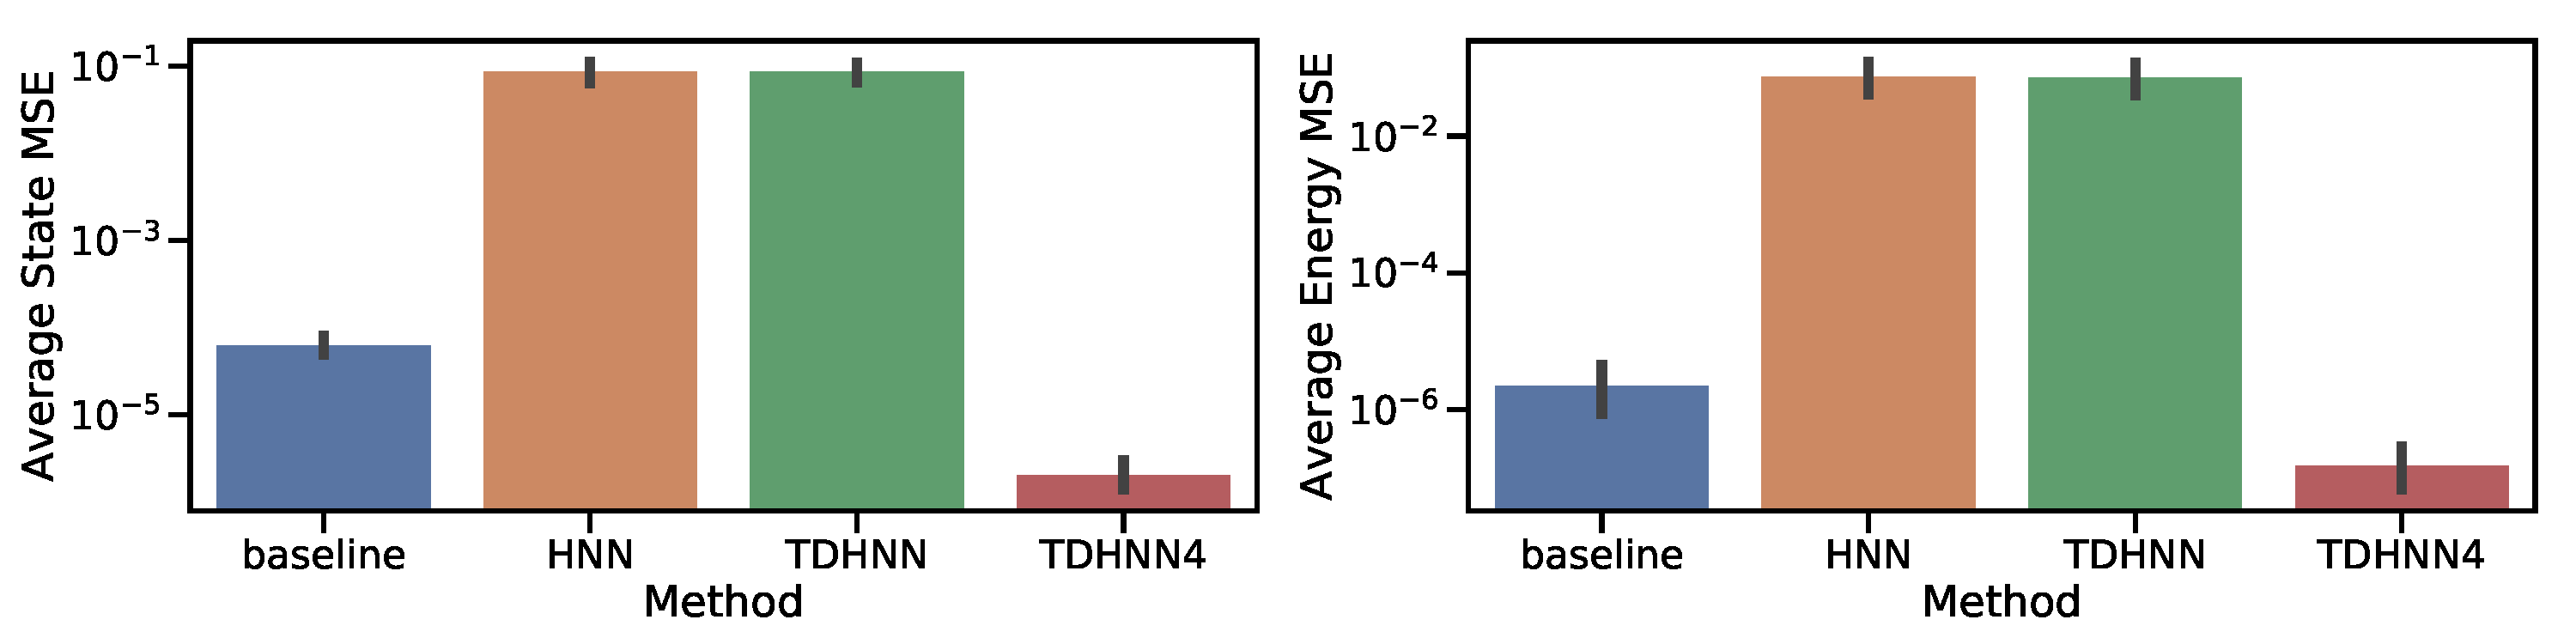
\includegraphics[width=\textwidth]{figures/figures/damped/1/damped_errors_0.pdf}
\caption{The average state and energy MSE across 25 test points}
\end{subfigure}
\begin{subfigure}[b]{0.48\textwidth}
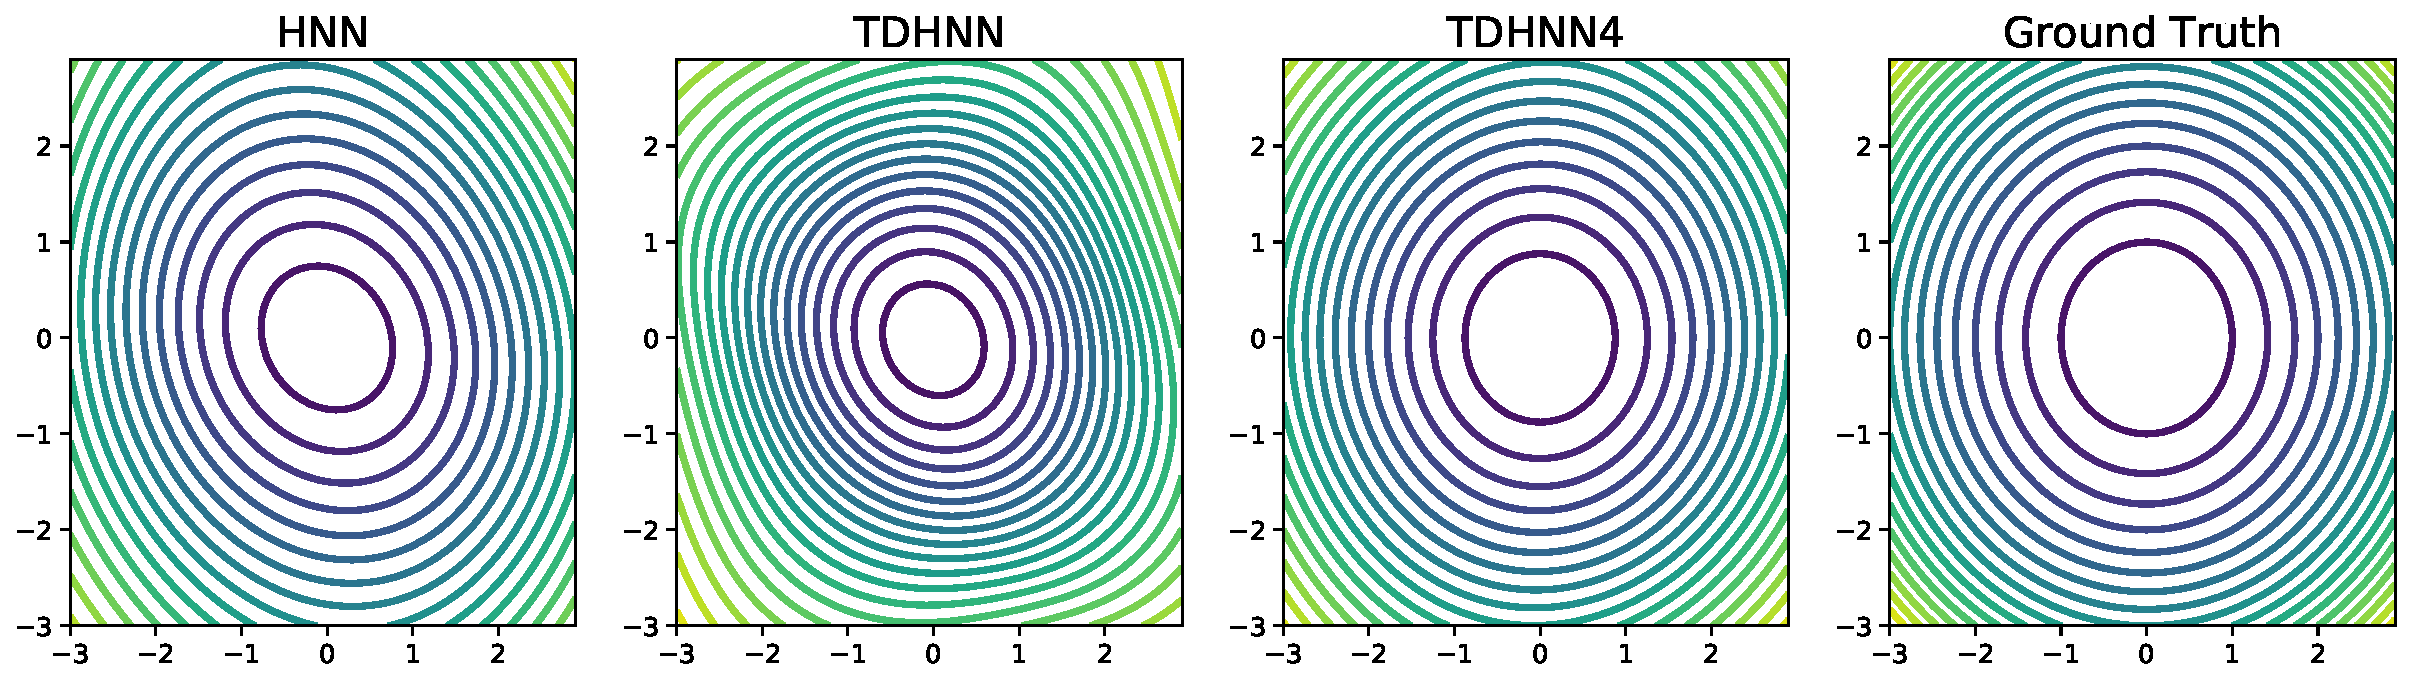
\includegraphics[width=\textwidth]{figures/figures/damped/1/damped_hamiltonian_0.pdf}
\caption{The learnt Hamiltonian across methods}
\end{subfigure}
\begin{subfigure}[b]{0.48\textwidth}
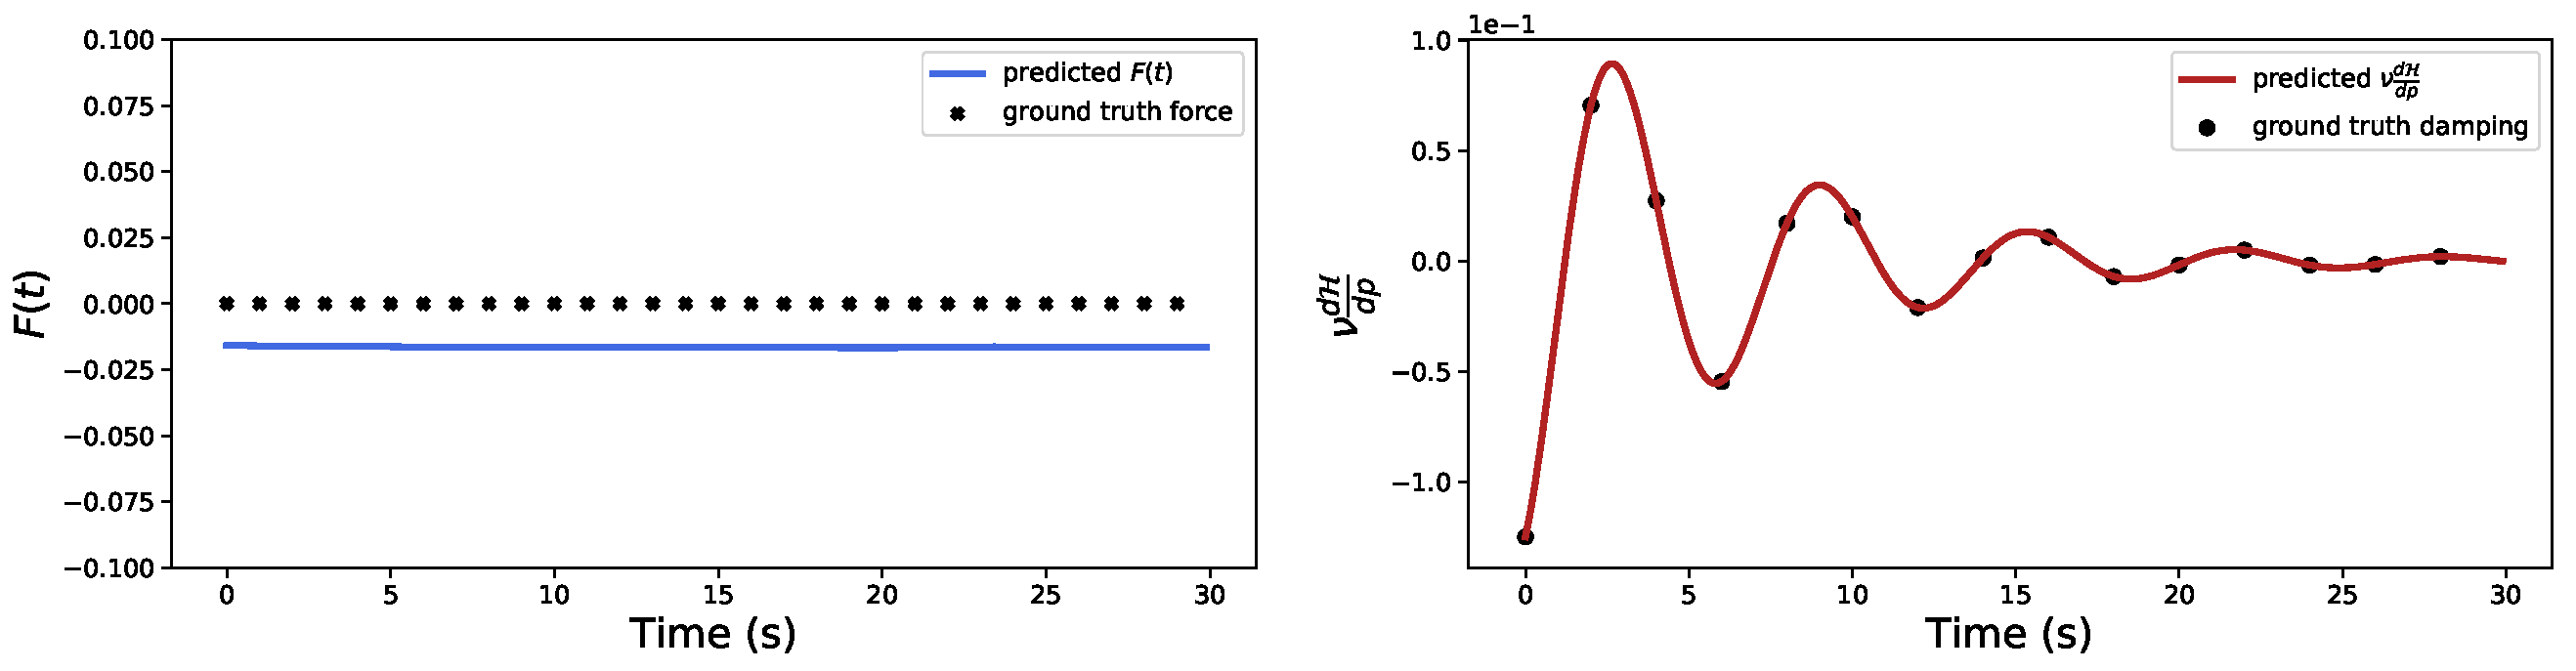
\includegraphics[width=\textwidth]{figures/figures/damped/1/damped_dpdt_new_0.pdf}
\caption{The learnt force and damping of TDHNN4}
\end{subfigure}
\label{mspring_full}
\end{figure}
\begin{figure}[!htb]
\centering
\captionsetup{justification=centering}
\begin{subfigure}[b]{0.48\textwidth}
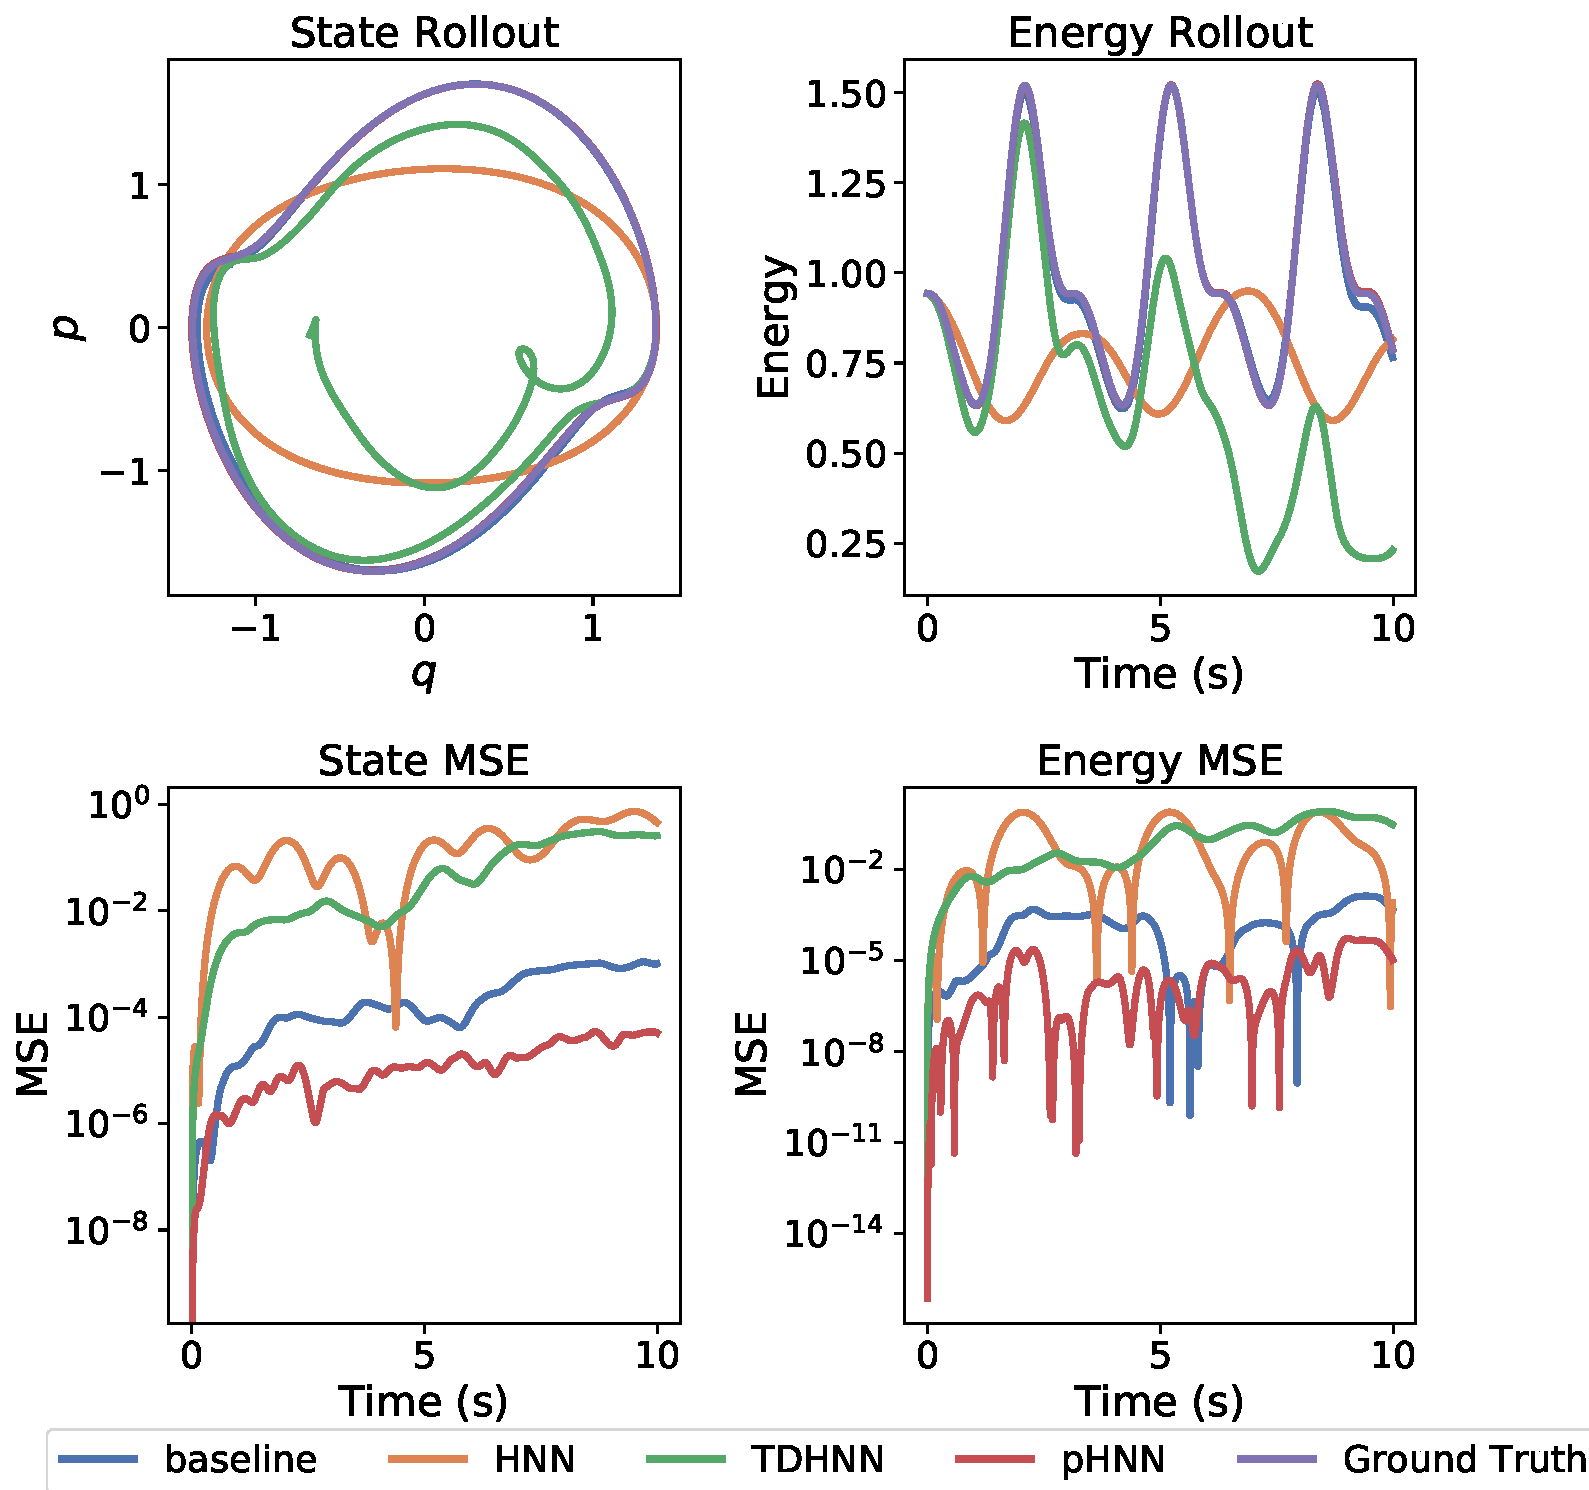
\includegraphics[width=\textwidth]{figures/figures/forced_mass_spring/1/forced_mass_spring_long_0.pdf}
\caption{State and energy rollout of an initial condition from the test set}
\end{subfigure}
\begin{subfigure}[b]{0.48\textwidth}
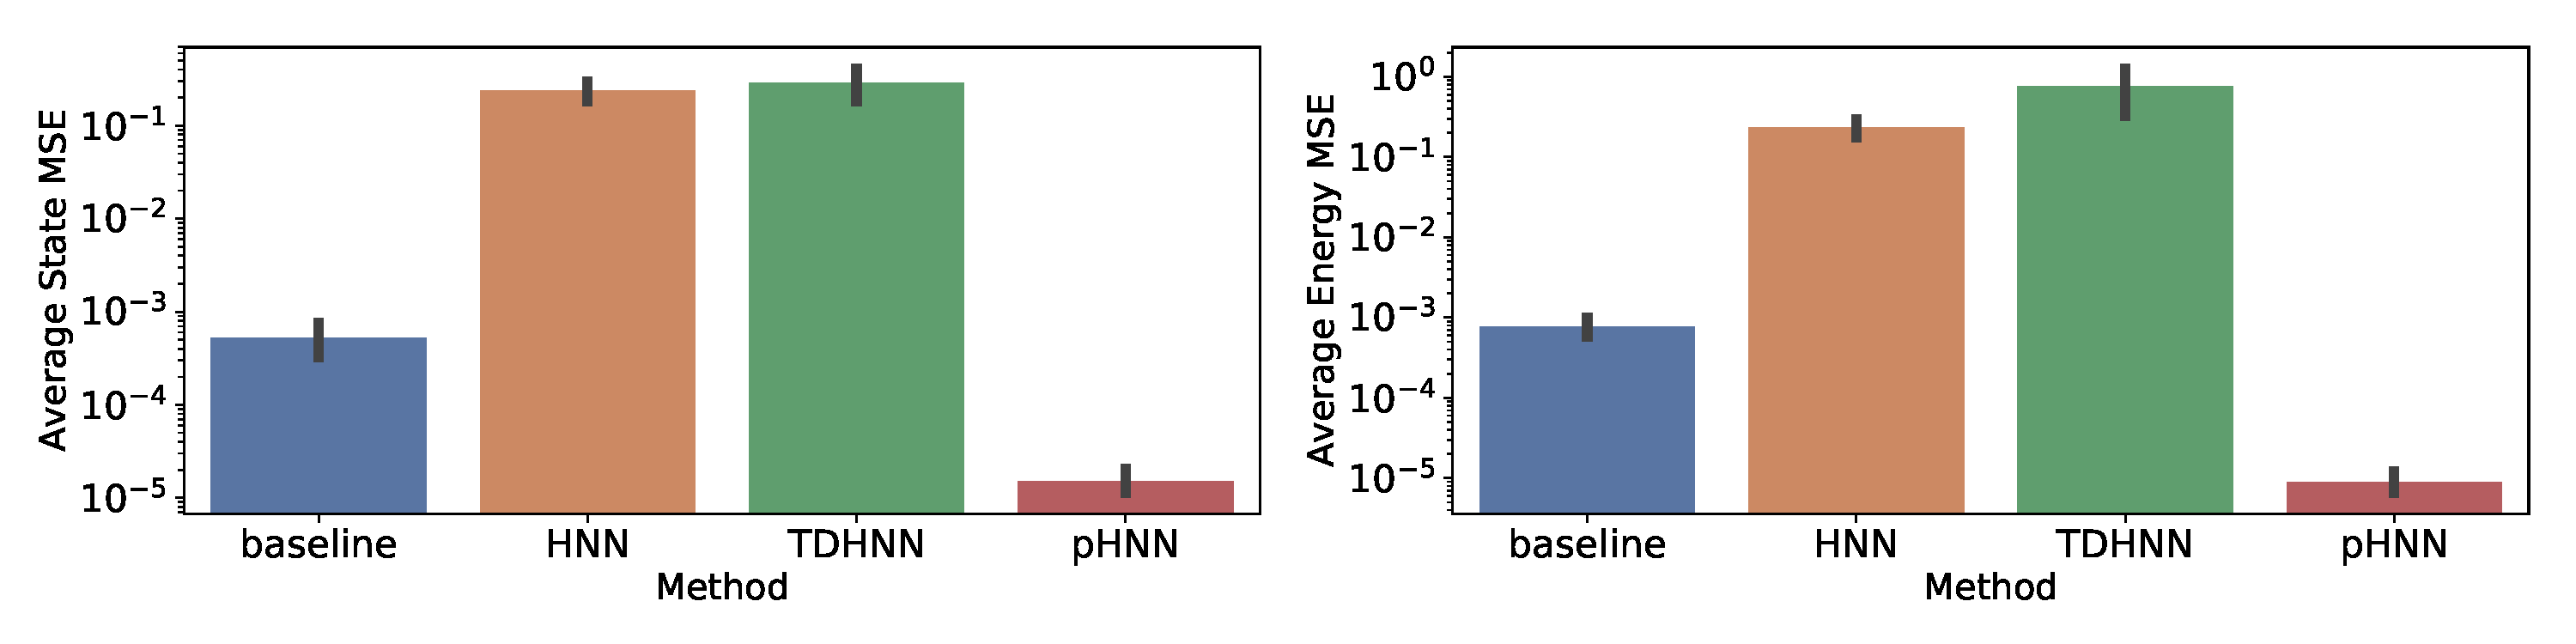
\includegraphics[width=\textwidth]{figures/figures/forced_mass_spring/1/forced_mass_spring_errors_0.pdf}
\caption{The average state and energy MSE across 25 test points}
\end{subfigure}
\begin{subfigure}[b]{0.48\textwidth}
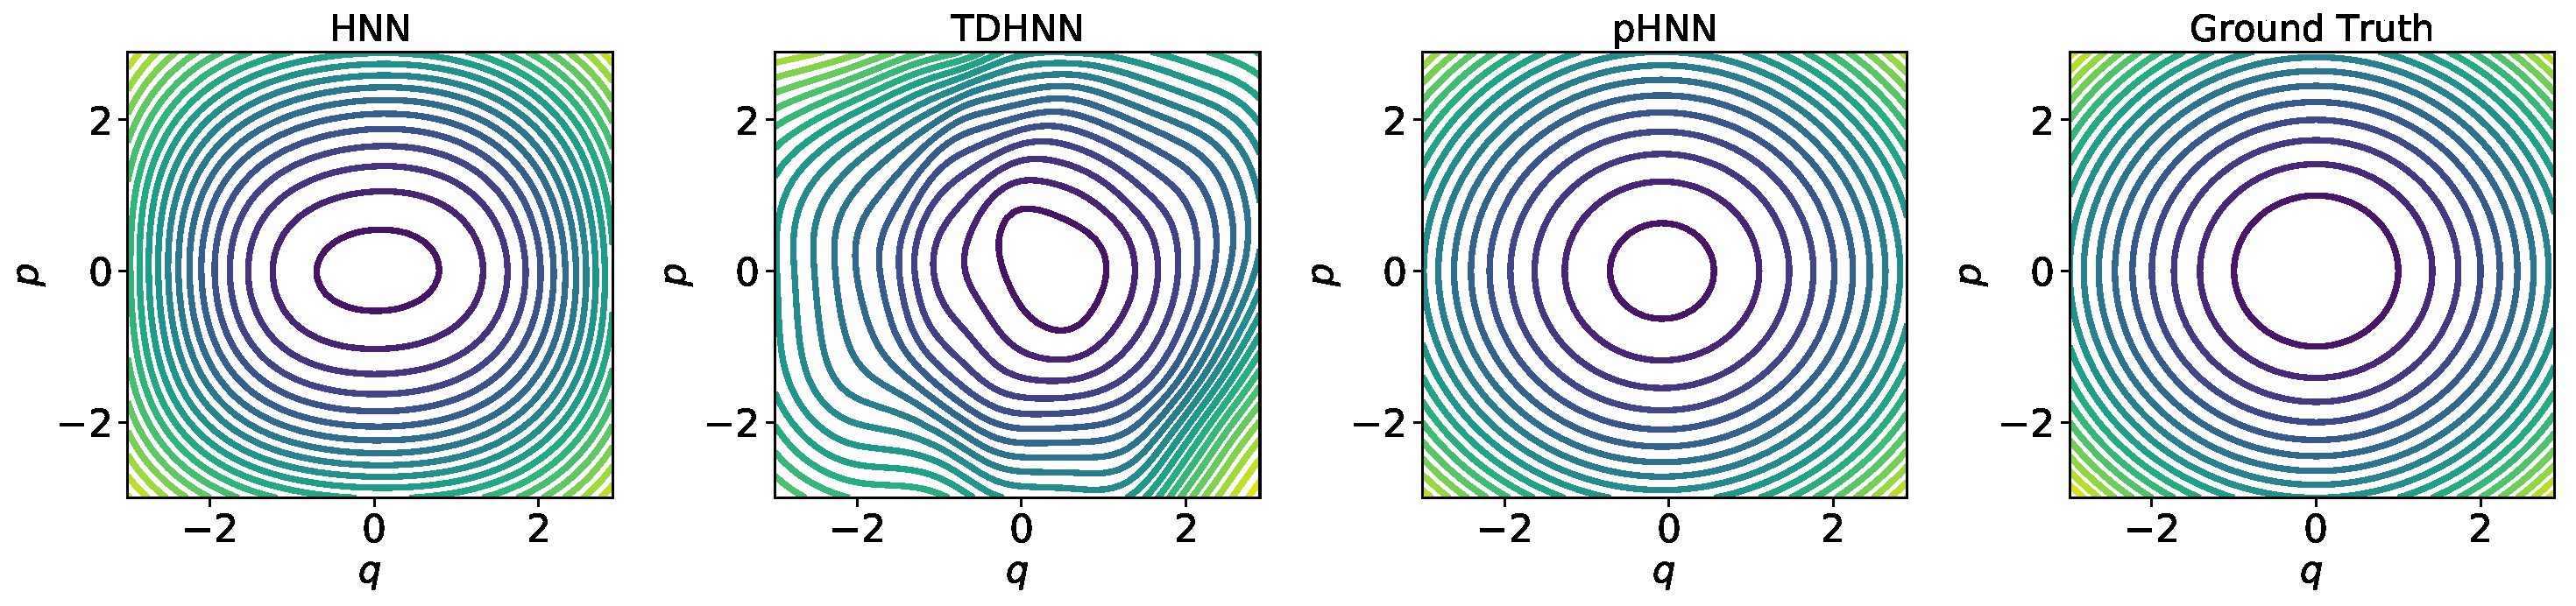
\includegraphics[width=\textwidth]{figures/figures/forced_mass_spring/1/forced_mass_spring_hamiltonian_0.pdf}
\caption{The learnt Hamiltonian across methods}
\end{subfigure}
\begin{subfigure}[b]{0.48\textwidth}
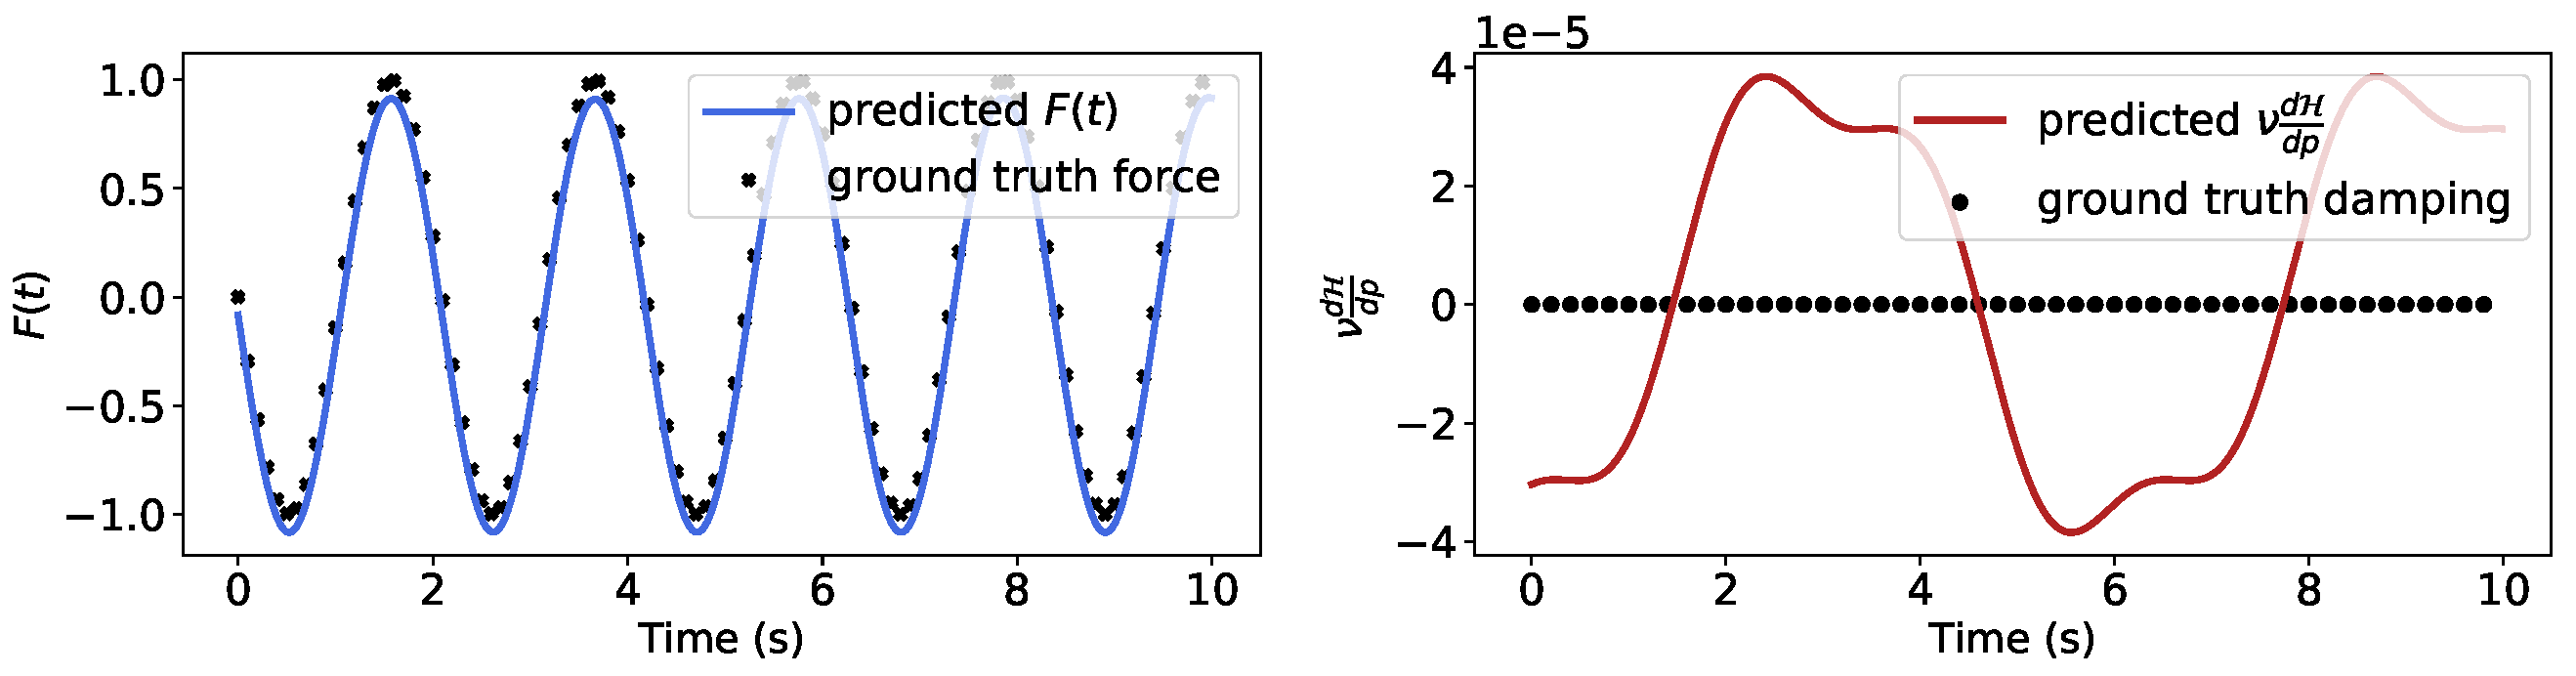
\includegraphics[width=\textwidth]{figures/figures/forced_mass_spring/1/forced_mass_spring_dpdt_new_0.pdf}
\caption{The learnt force and damping of TDHNN4}
\end{subfigure}
\label{forced_mspring_1_full}
\end{figure}
\begin{figure}[!htb]
\centering
\captionsetup{justification=centering}
\begin{subfigure}[b]{0.48\textwidth}
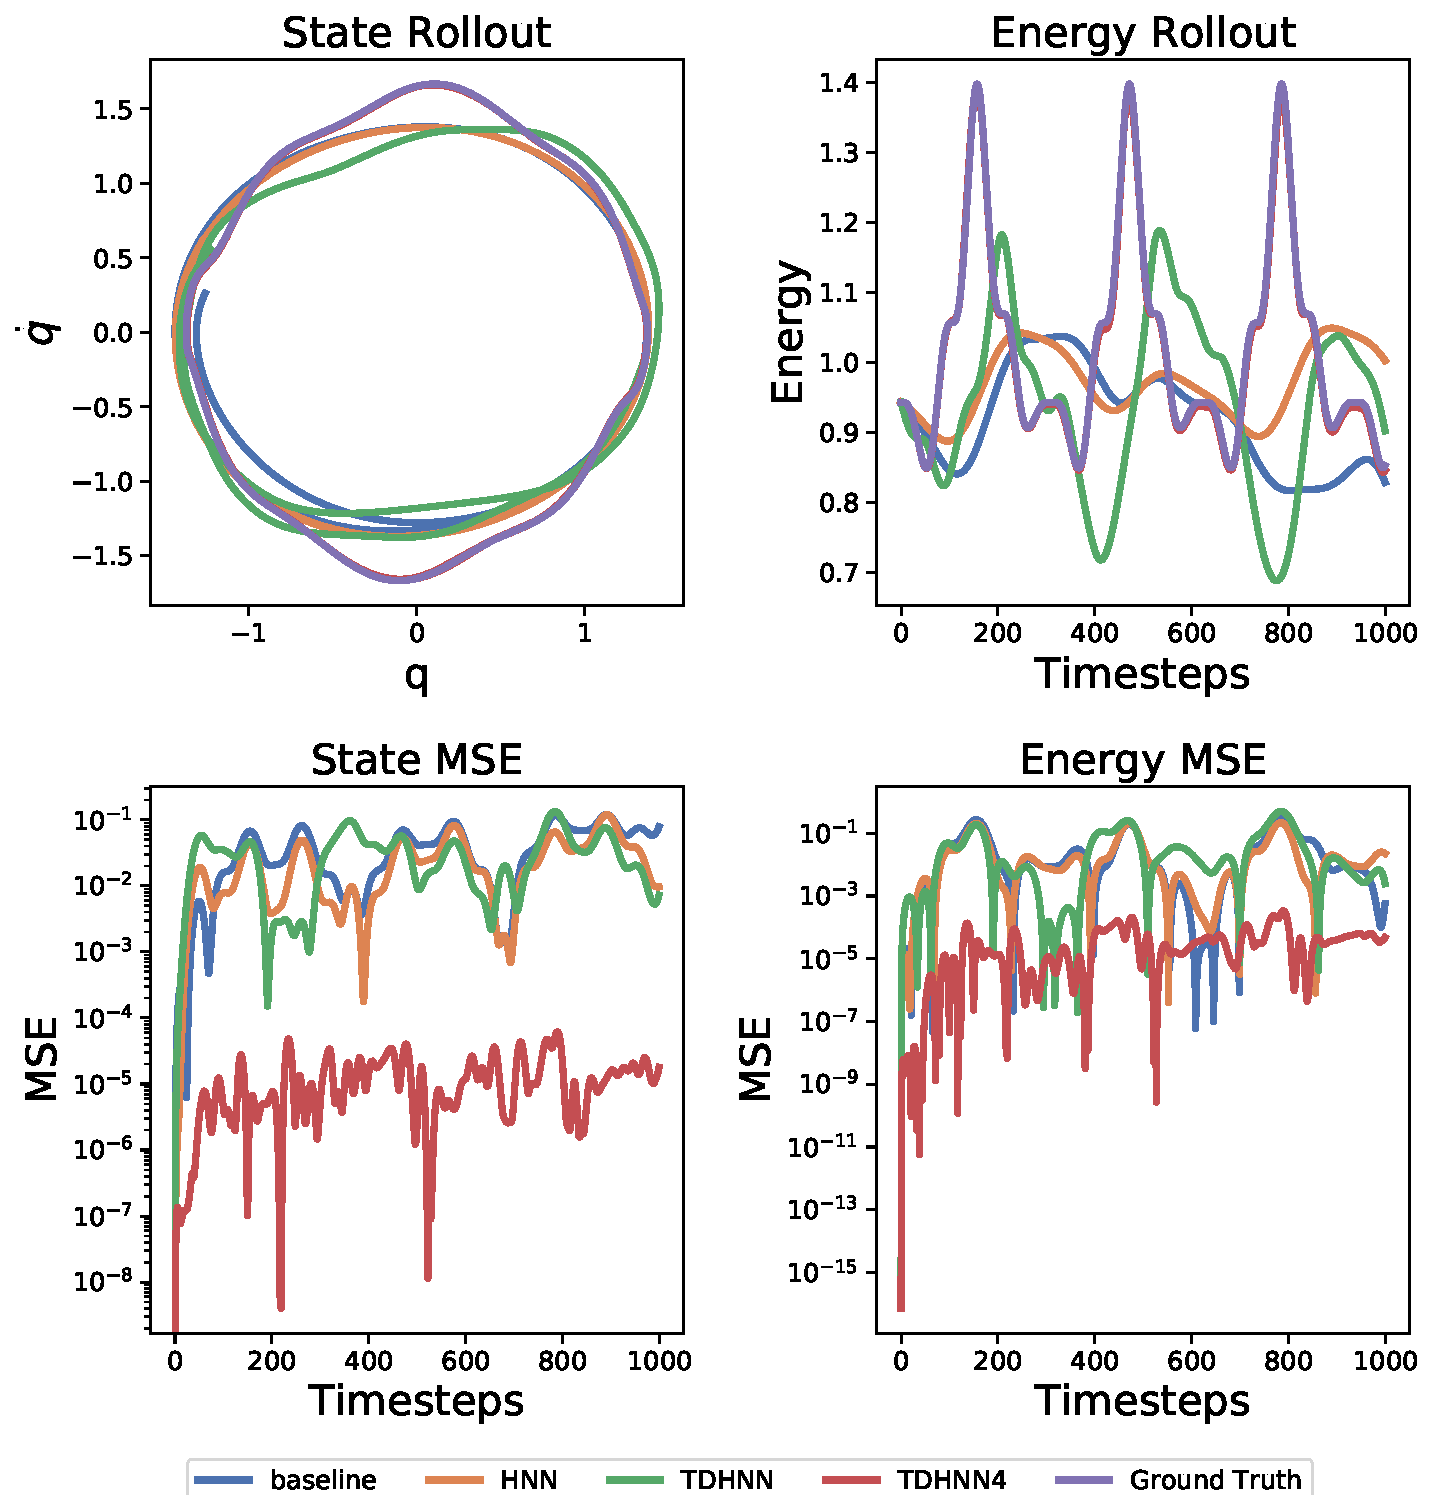
\includegraphics[width=\textwidth]{figures/figures/forced_mass_spring/2/forced_mass_spring_long_0.pdf}
\caption{State and energy rollout of an initial condition from the test set}
\end{subfigure}
\begin{subfigure}[b]{0.48\textwidth}
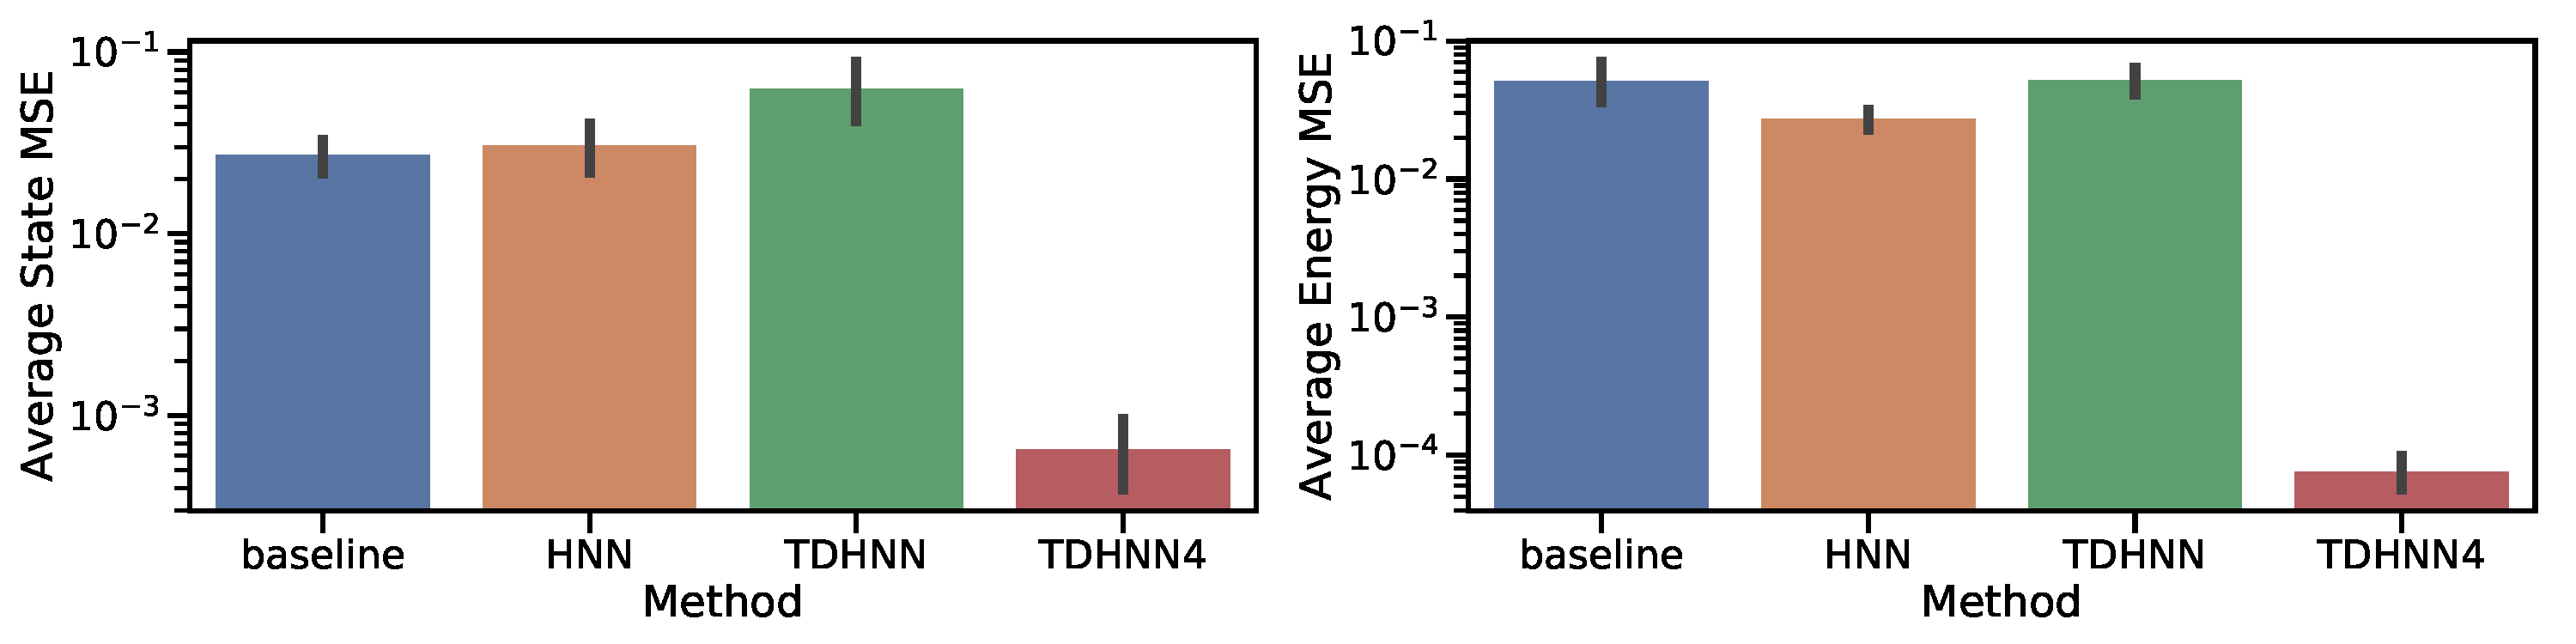
\includegraphics[width=\textwidth]{figures/figures/forced_mass_spring/2/forced_mass_spring_errors_0.pdf}
\caption{The average state and energy MSE across 25 test points}
\end{subfigure}
\begin{subfigure}[b]{0.48\textwidth}
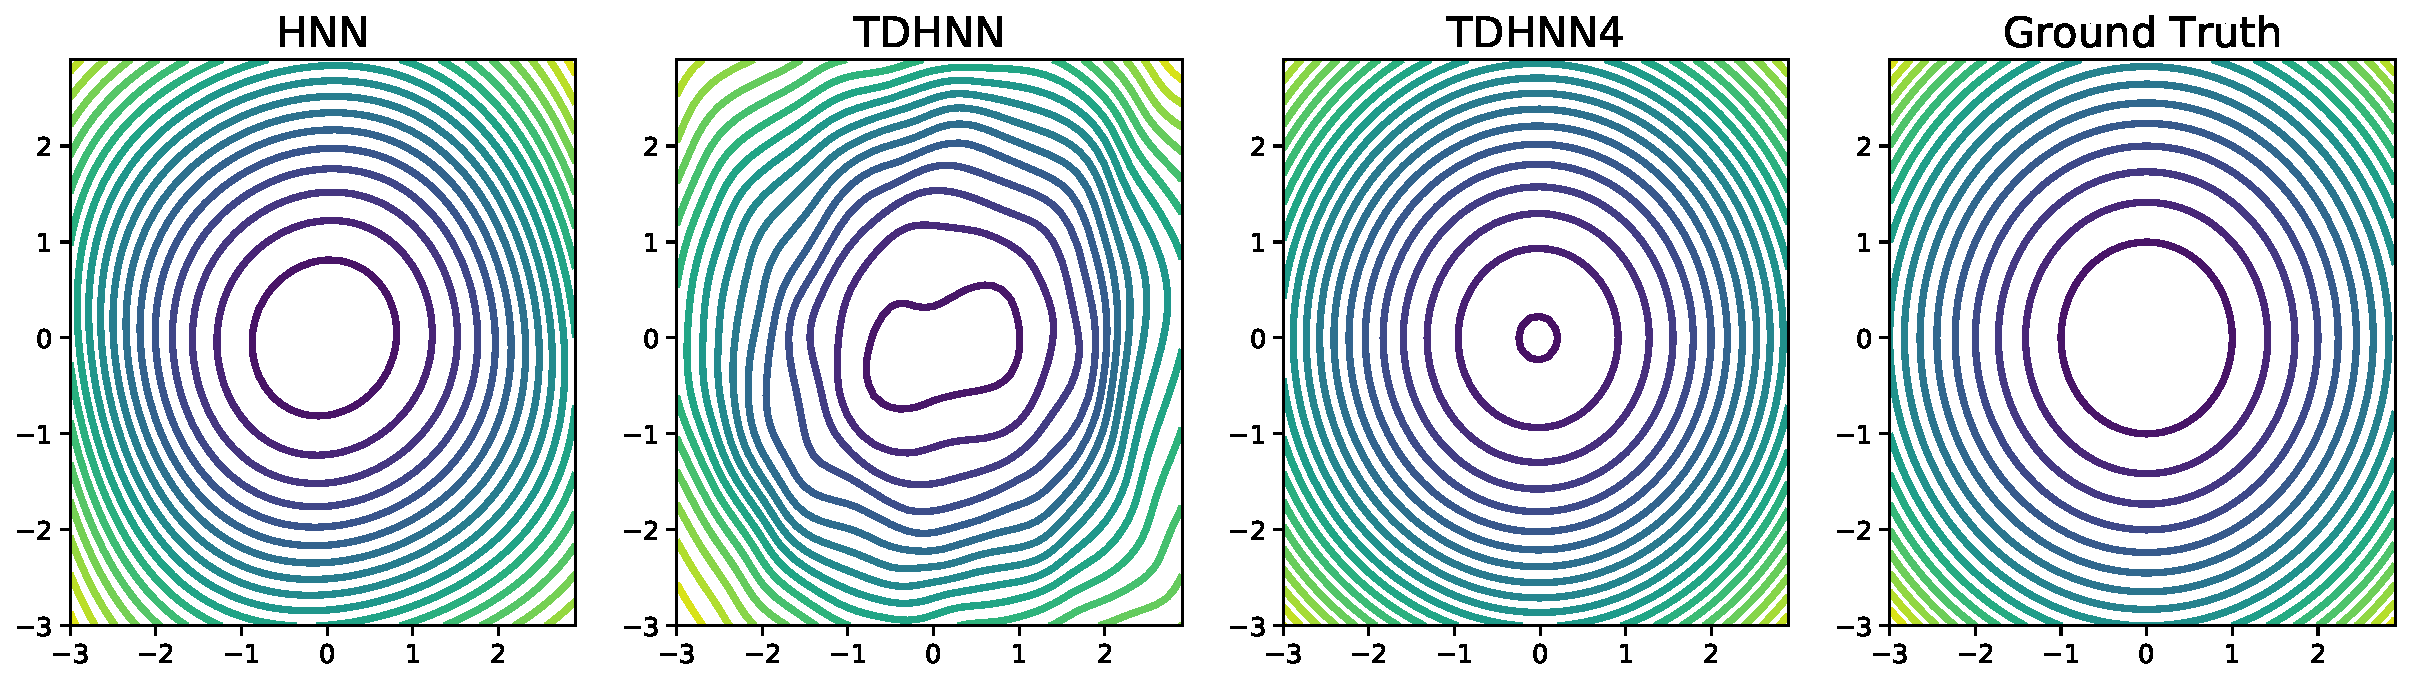
\includegraphics[width=\textwidth]{figures/figures/forced_mass_spring/2/forced_mass_spring_hamiltonian_0.pdf}
\caption{The learnt Hamiltonian across methods}
\end{subfigure}
\begin{subfigure}[b]{0.48\textwidth}
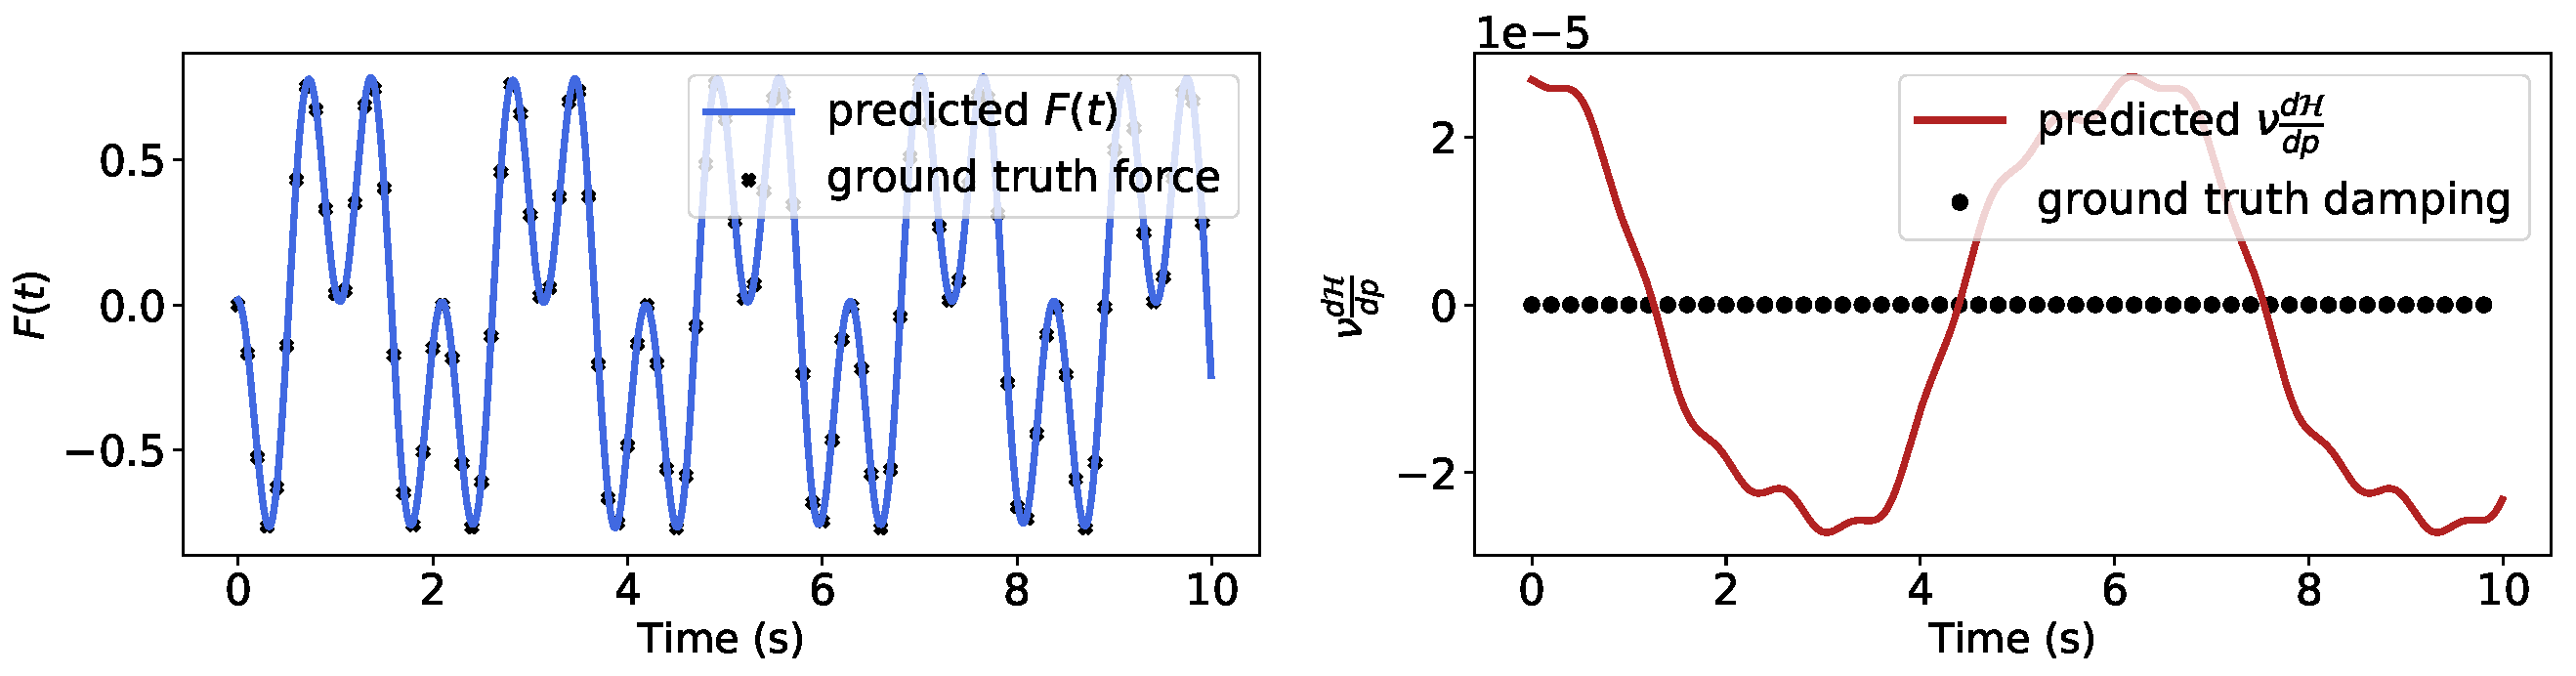
\includegraphics[width=\textwidth]{figures/figures/forced_mass_spring/2/forced_mass_spring_dpdt_new_0.pdf}
\caption{The learnt force and damping of TDHNN4}
\end{subfigure}
\label{forced_mpsring_2_full}
\end{figure}
\begin{figure}[!htb]
\centering
\captionsetup{justification=centering}
\begin{subfigure}[b]{0.48\textwidth}
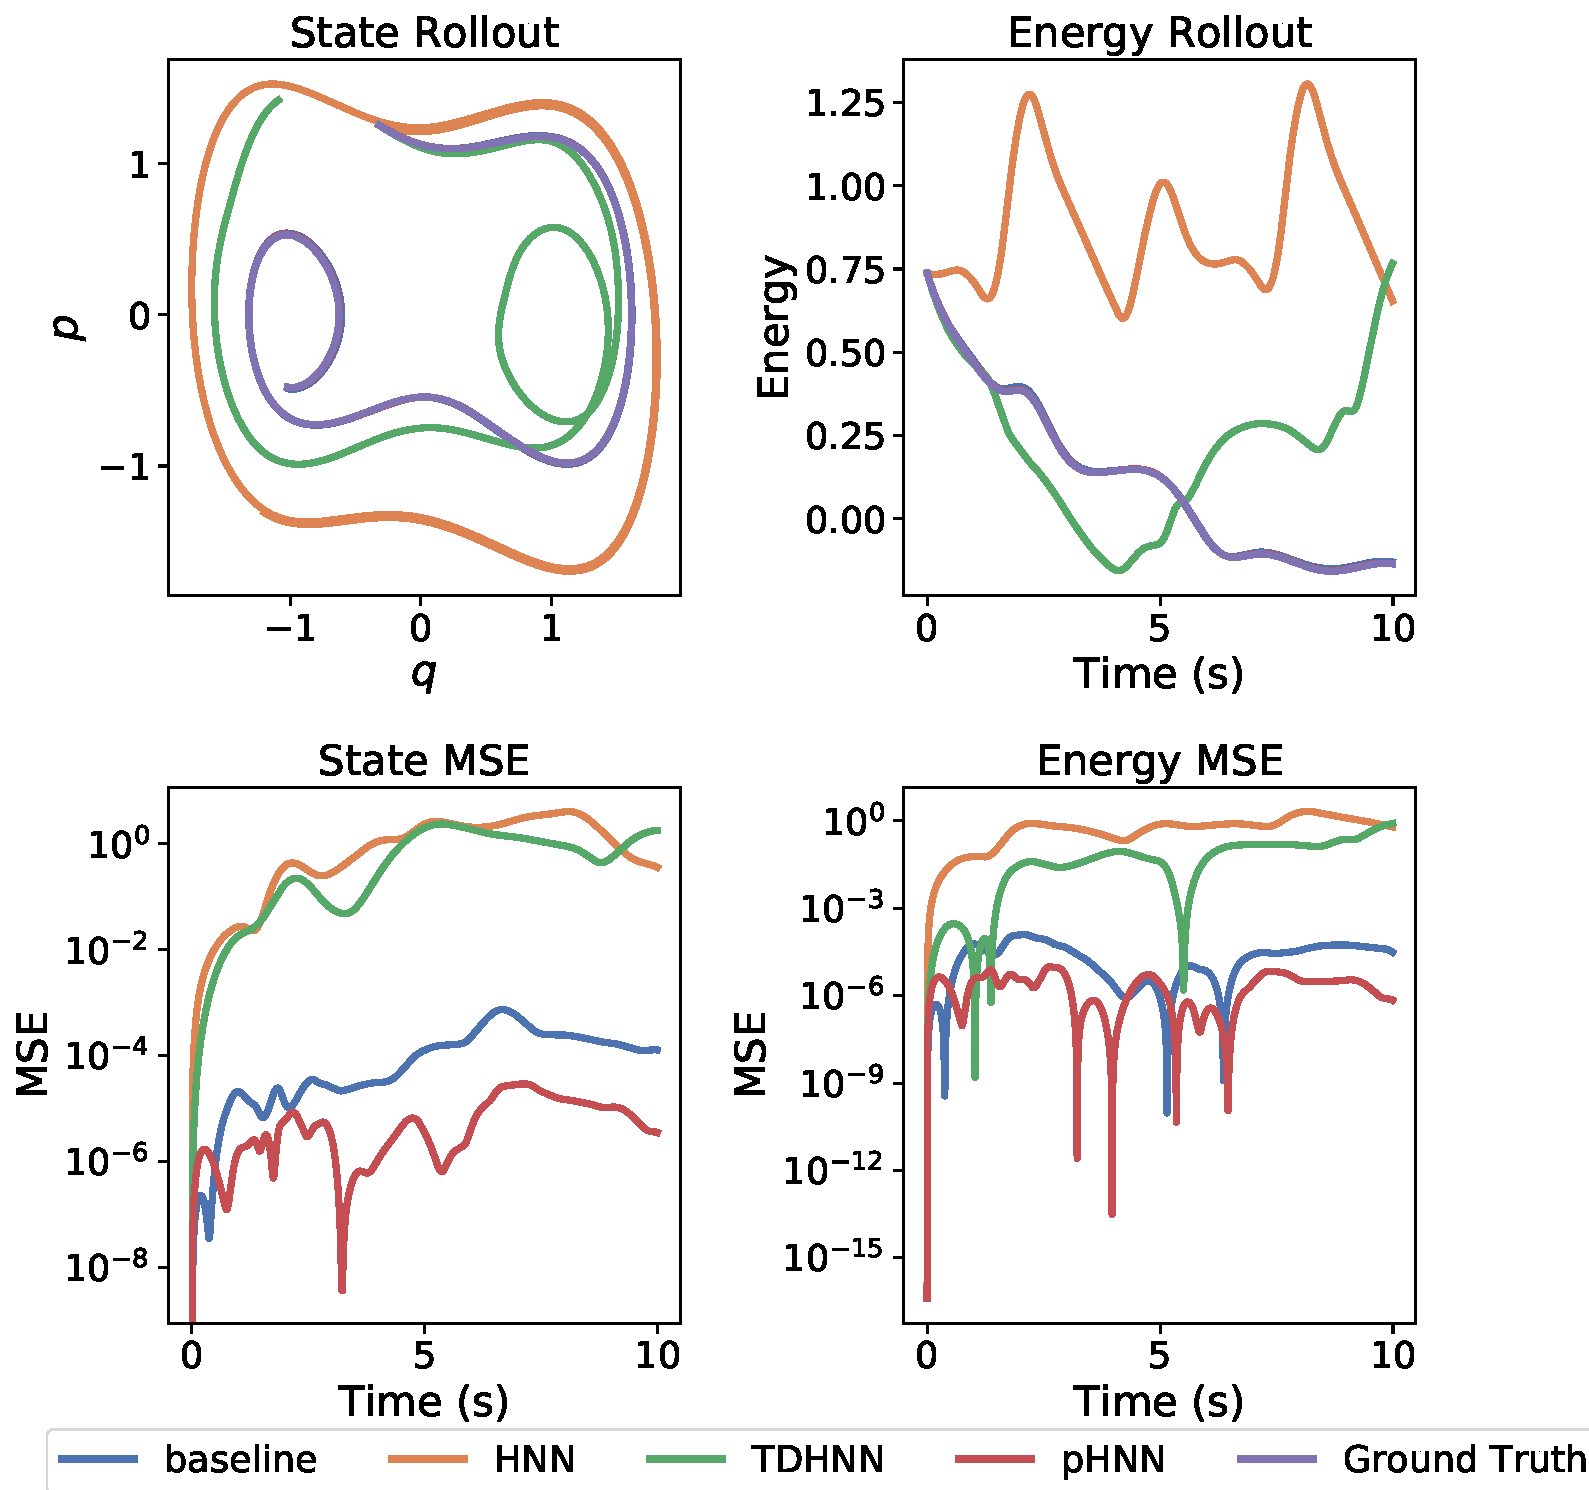
\includegraphics[width=\textwidth]{figures/figures/duffing/1/duffing_long_0.pdf}
\caption{State and energy rollout of an initial condition from the test set}
\end{subfigure}
\begin{subfigure}[b]{0.48\textwidth}
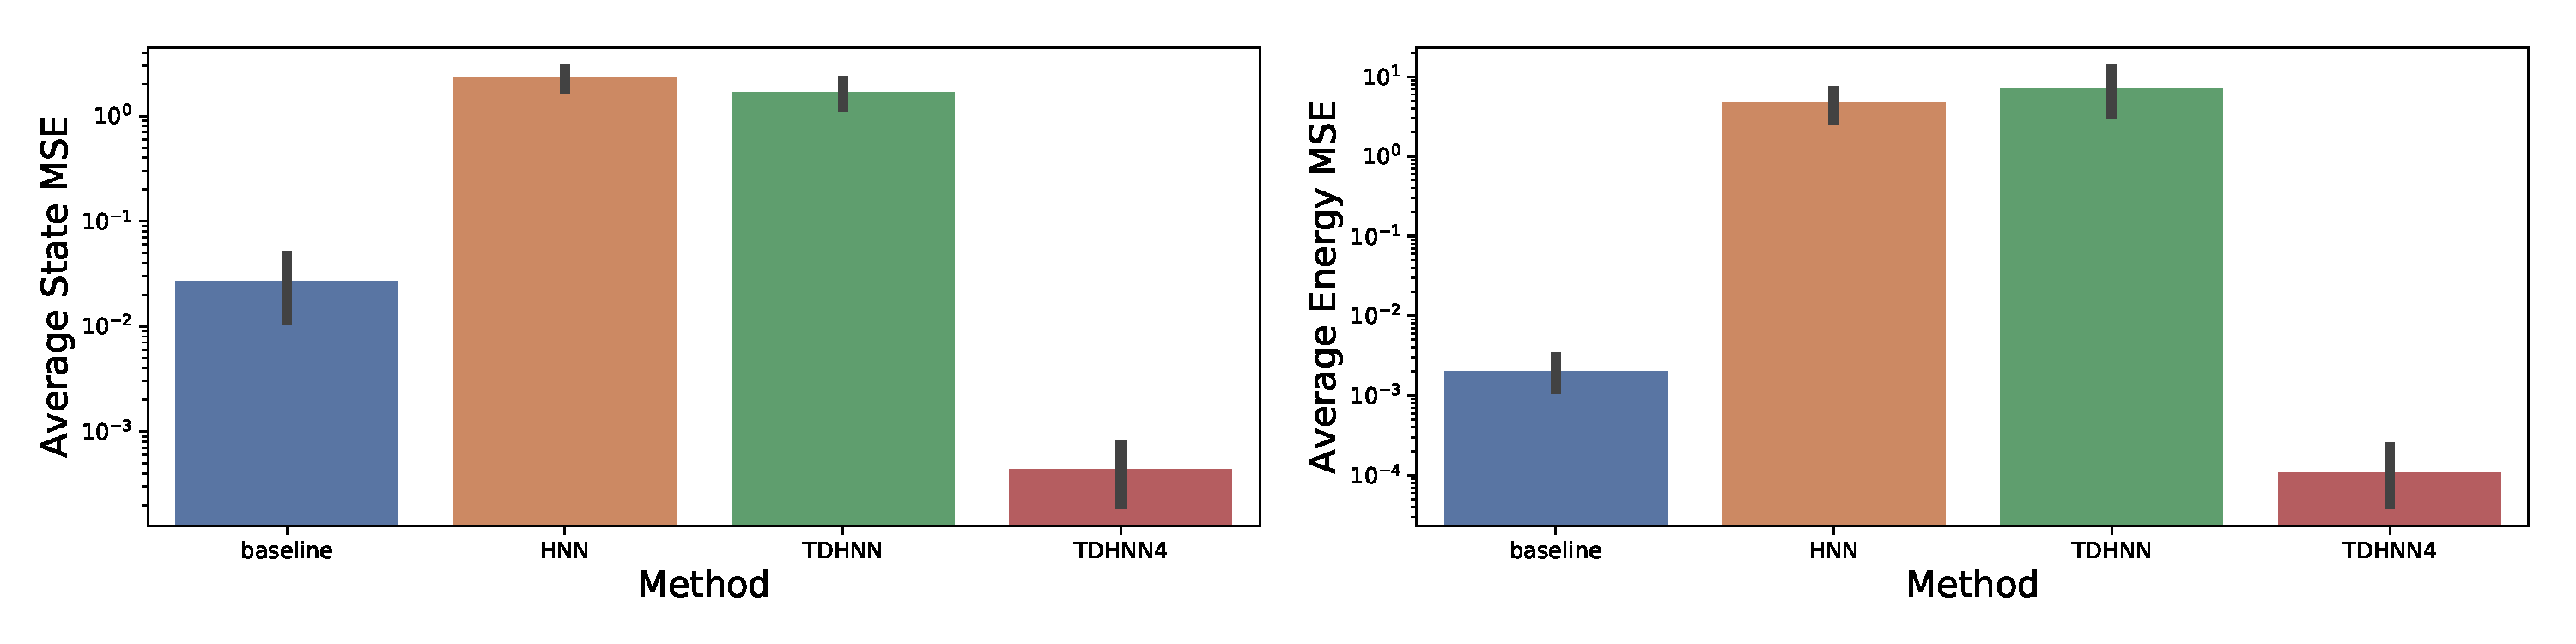
\includegraphics[width=\textwidth]{figures/figures/duffing/1/duffing_errors_0.pdf}
\caption{The average state and energy MSE across 25 test points}
\end{subfigure}
\begin{subfigure}[b]{0.48\textwidth}
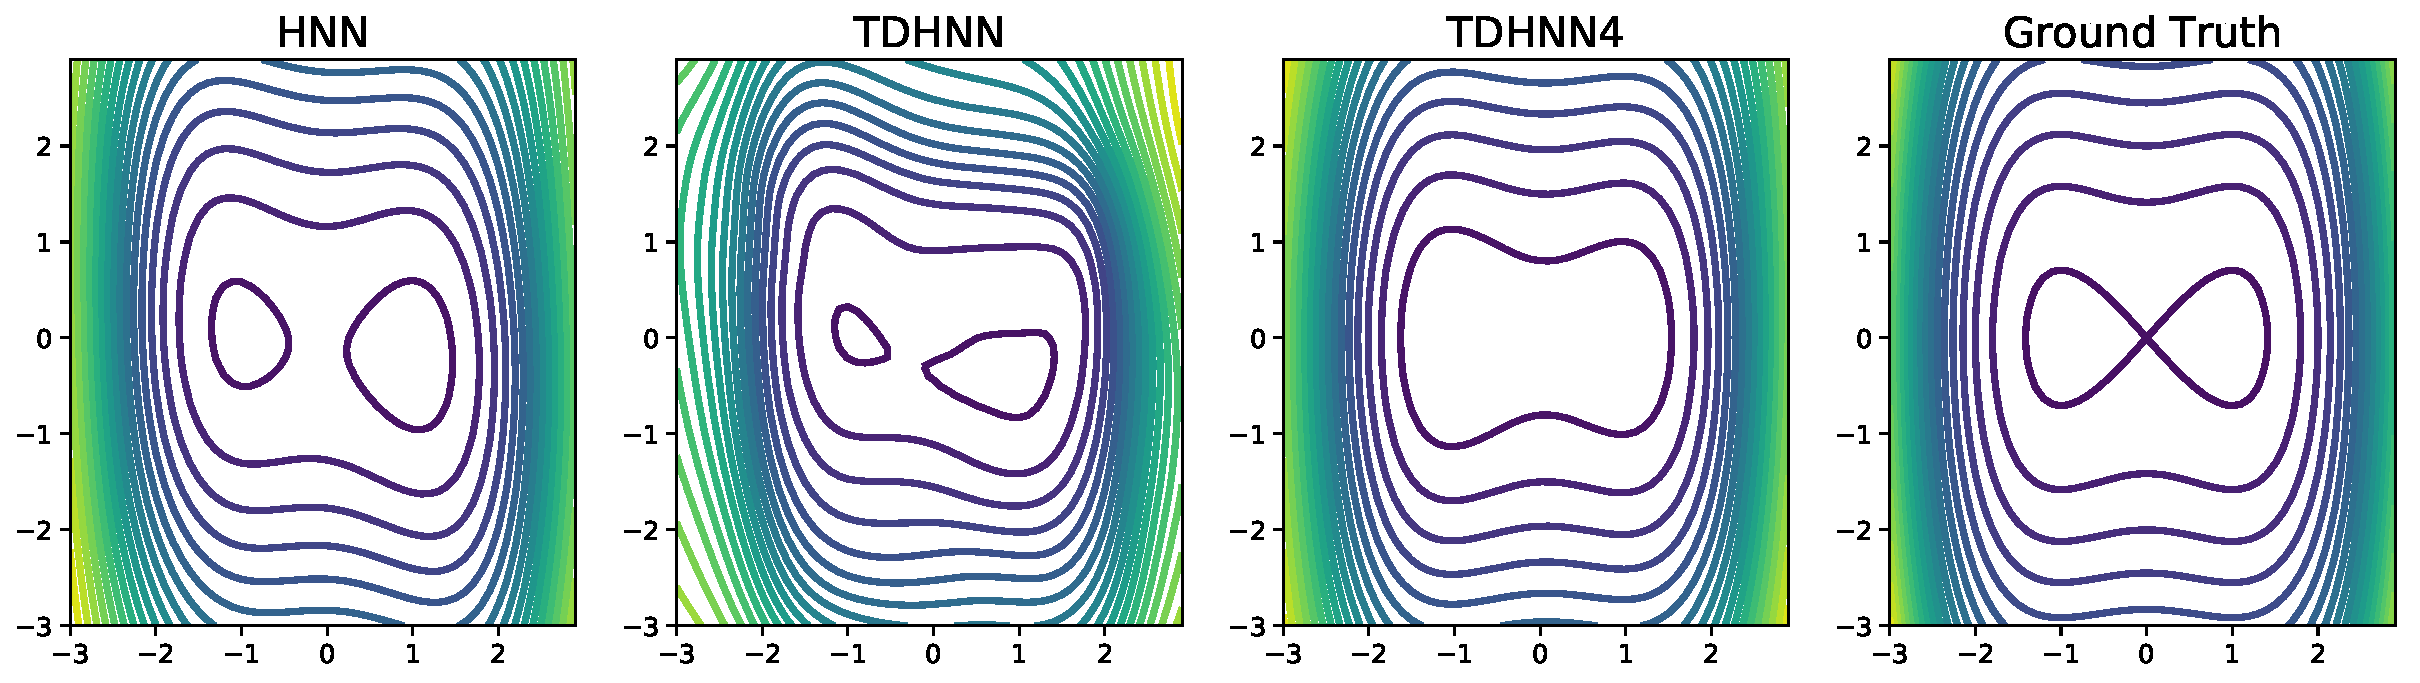
\includegraphics[width=\textwidth]{figures/figures/duffing/1/duffing_hamiltonian_0.pdf}
\caption{The learnt Hamiltonian across methods}
\end{subfigure}
\begin{subfigure}[b]{0.48\textwidth}
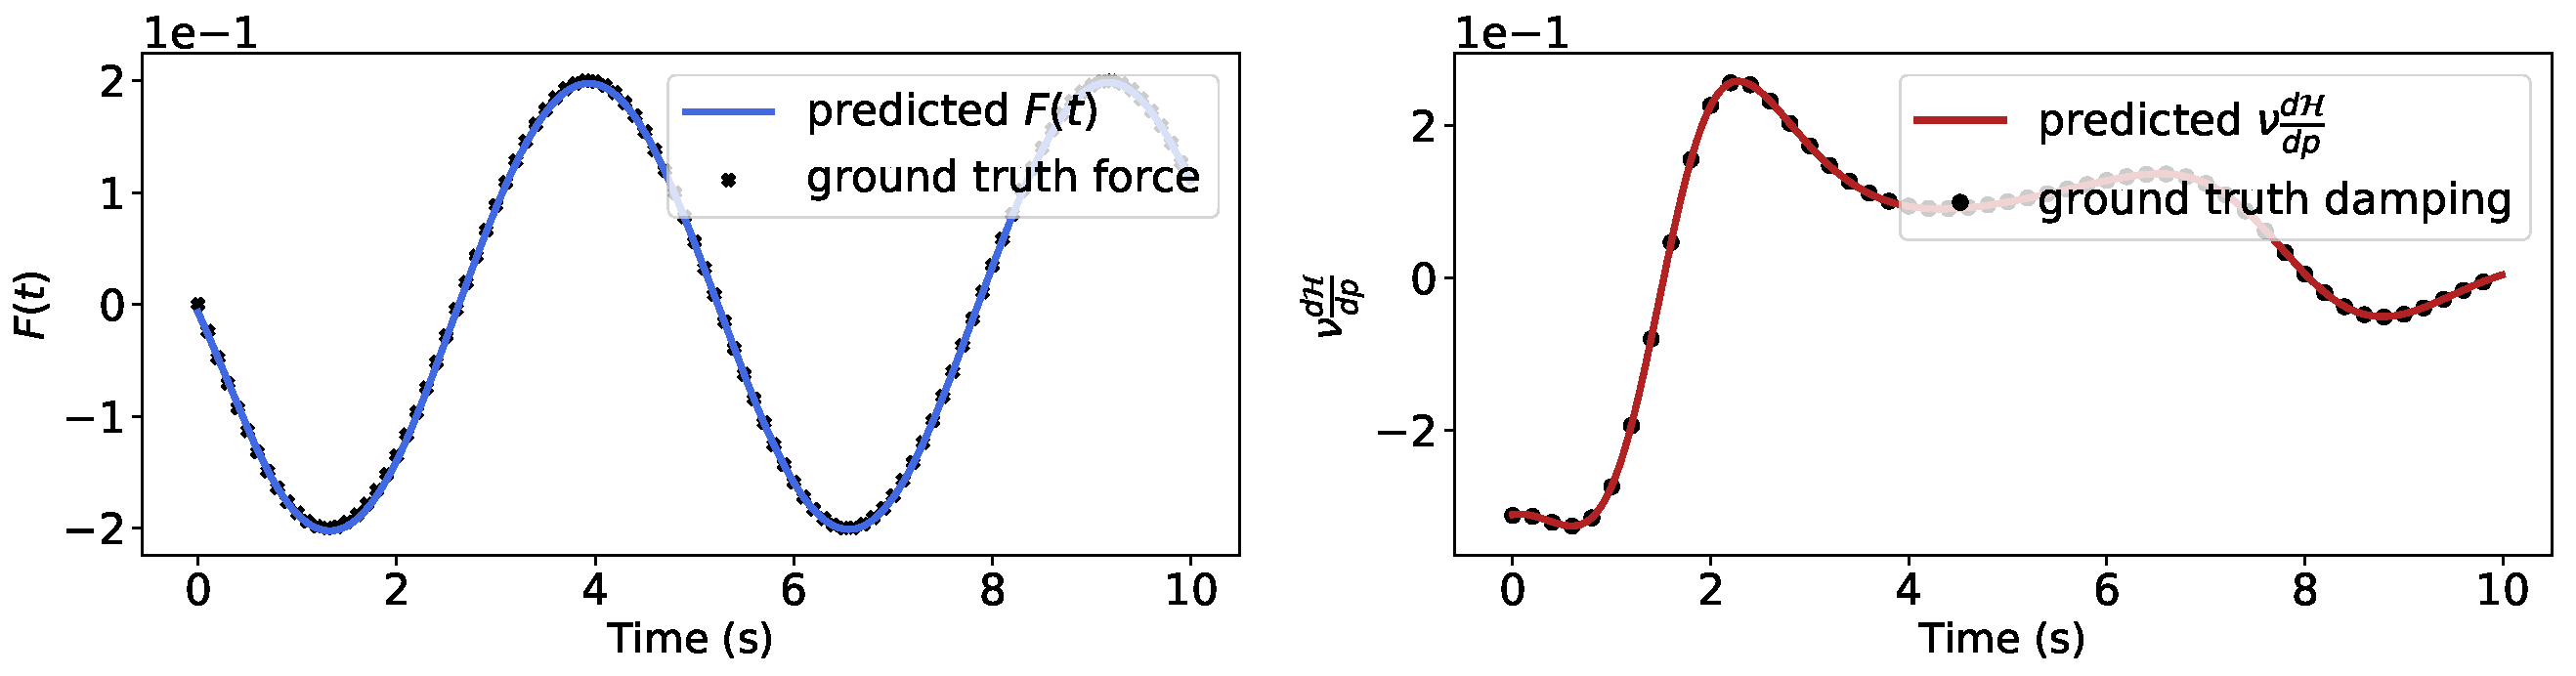
\includegraphics[width=\textwidth]{figures/figures/duffing/1/duffing_dpdt_new_0.pdf}
\caption{The learnt force and damping of TDHNN4}
\end{subfigure}
\label{duffing_1_full}
\end{figure}
\begin{figure}[!htb]
\centering
\captionsetup{justification=centering}
\begin{subfigure}[b]{0.48\textwidth}
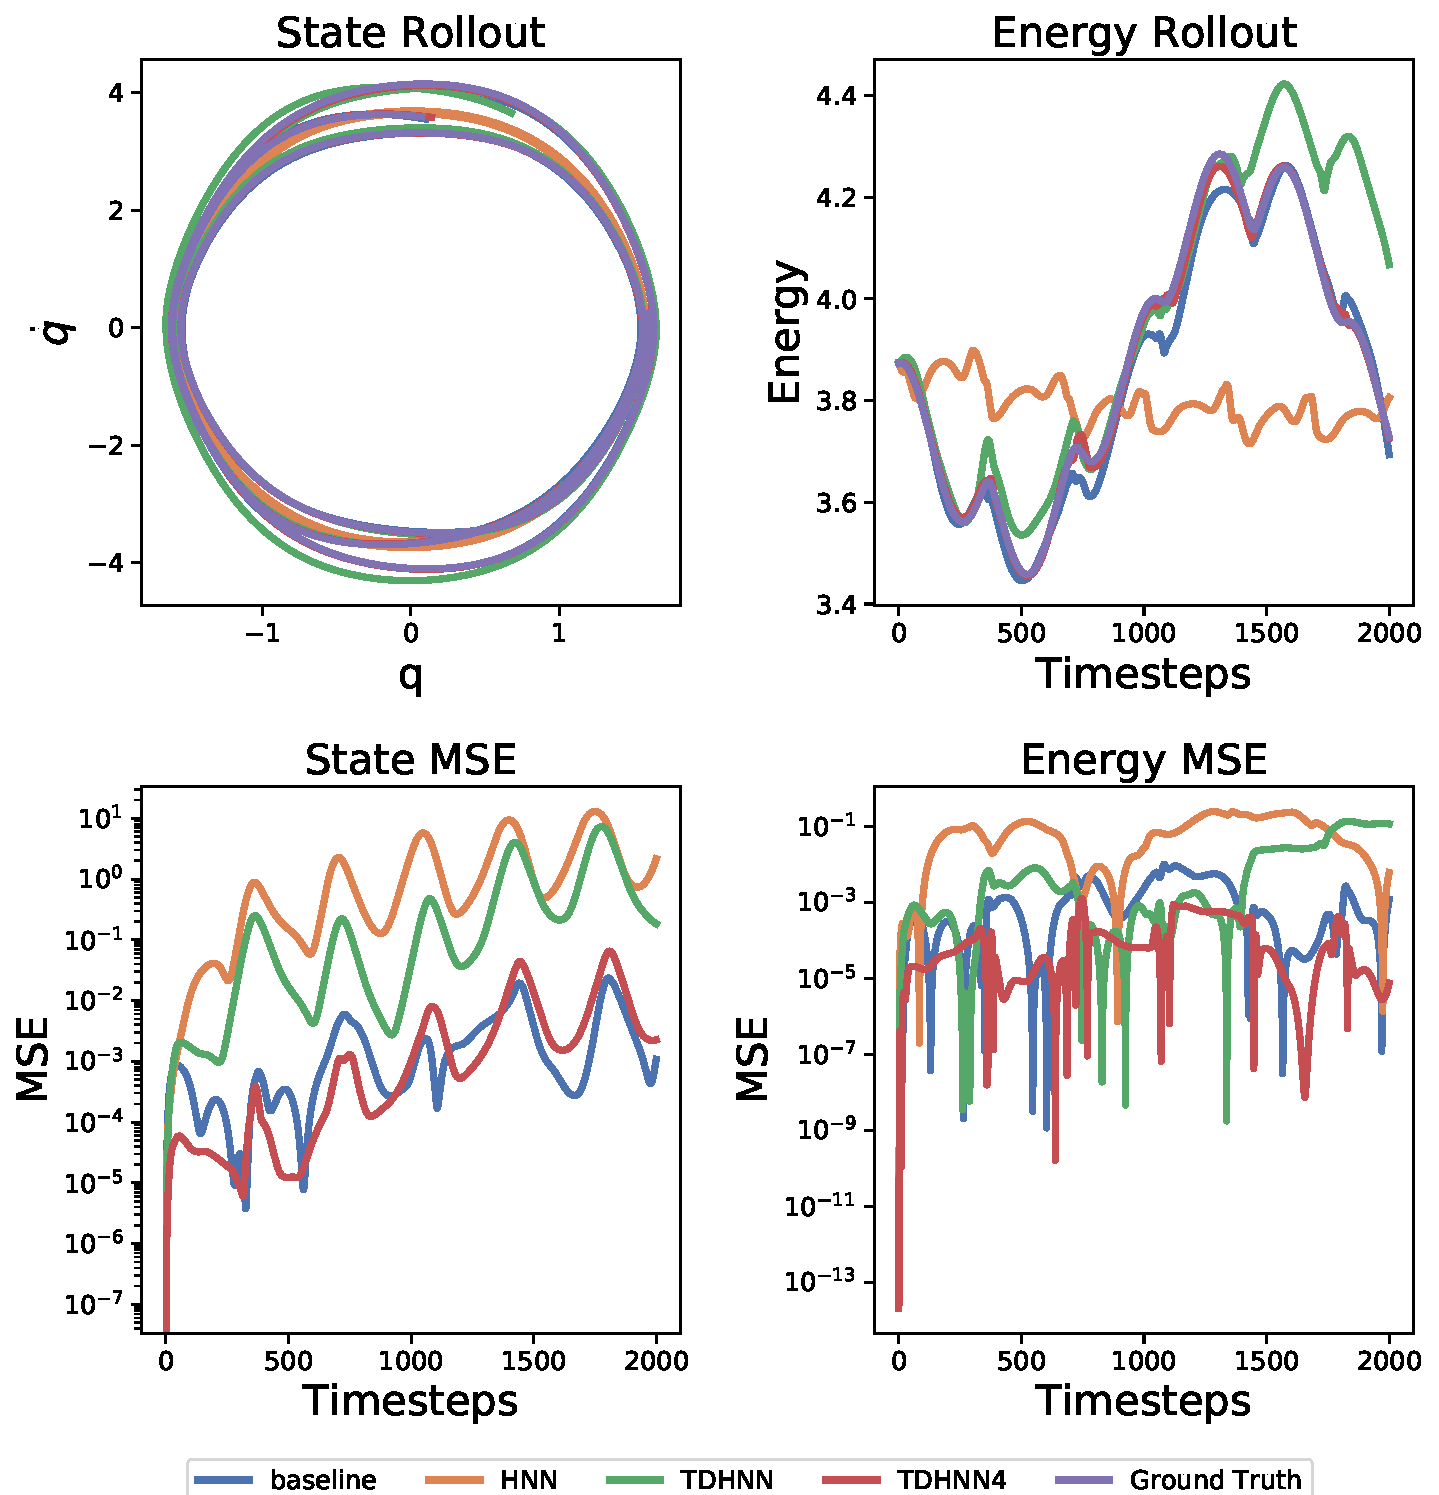
\includegraphics[width=\textwidth]{figures/figures/relativity/1/relativity_long_0.pdf}
\caption{State and energy rollout of an initial condition from the test set}
\end{subfigure}
\begin{subfigure}[b]{0.48\textwidth}
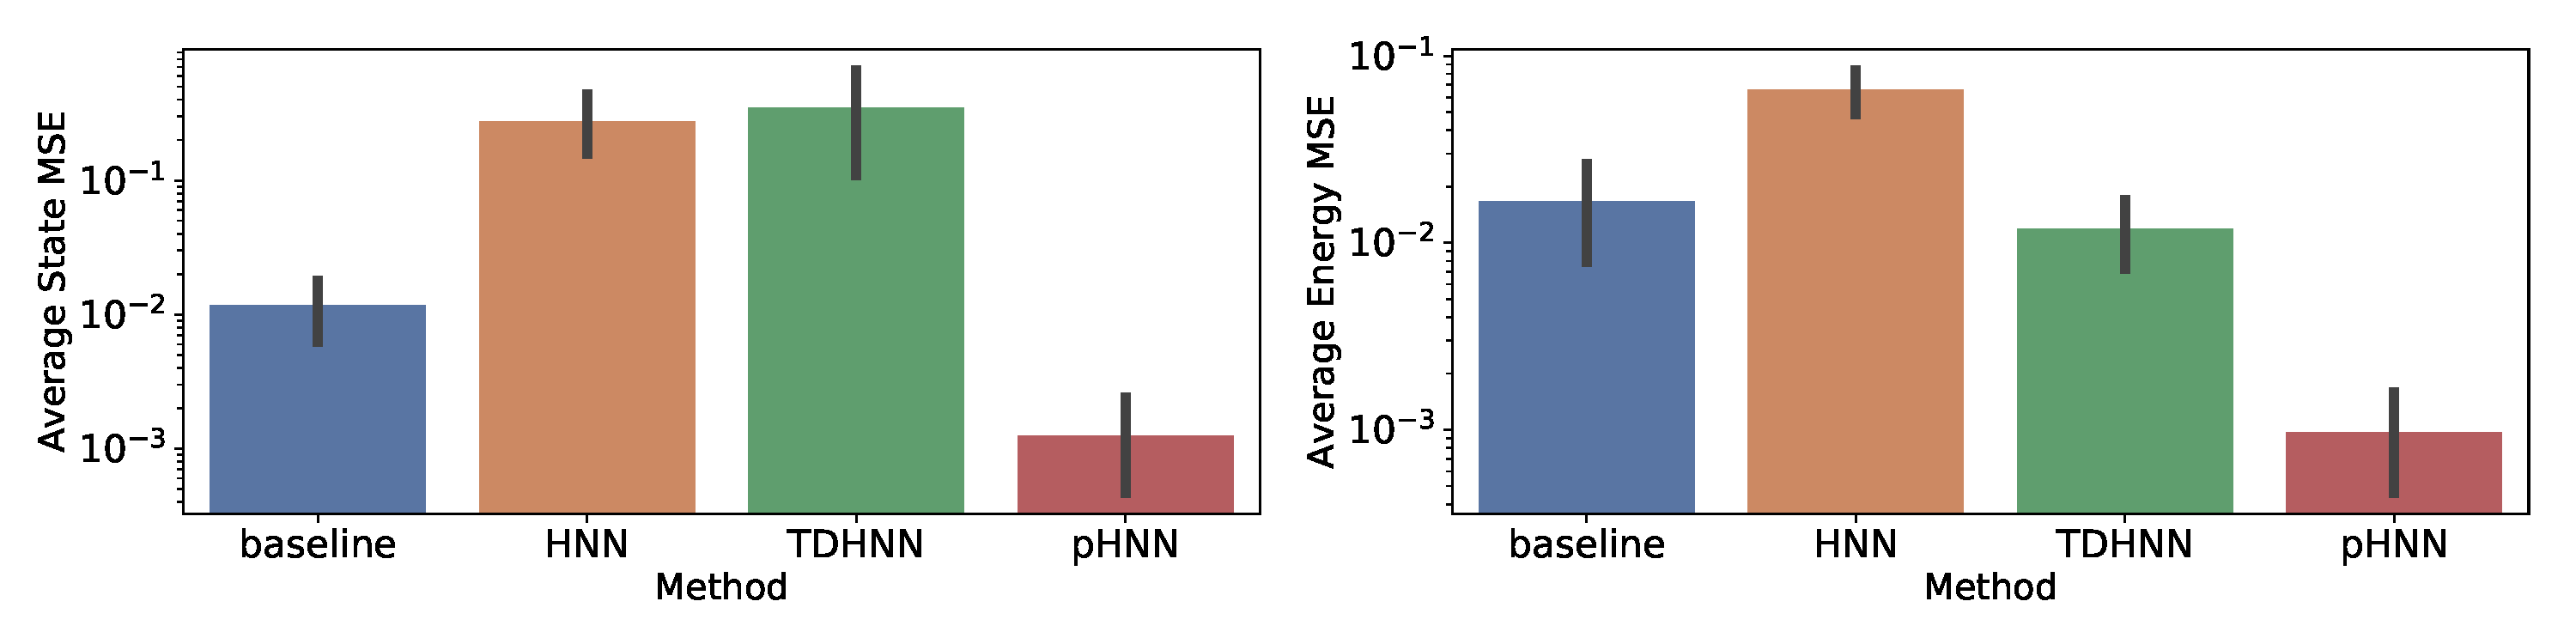
\includegraphics[width=\textwidth]{figures/figures/relativity/1/relativity_errors_0.pdf}
\caption{The average state and energy MSE across 25 test points}
\end{subfigure}
\begin{subfigure}[b]{0.48\textwidth}
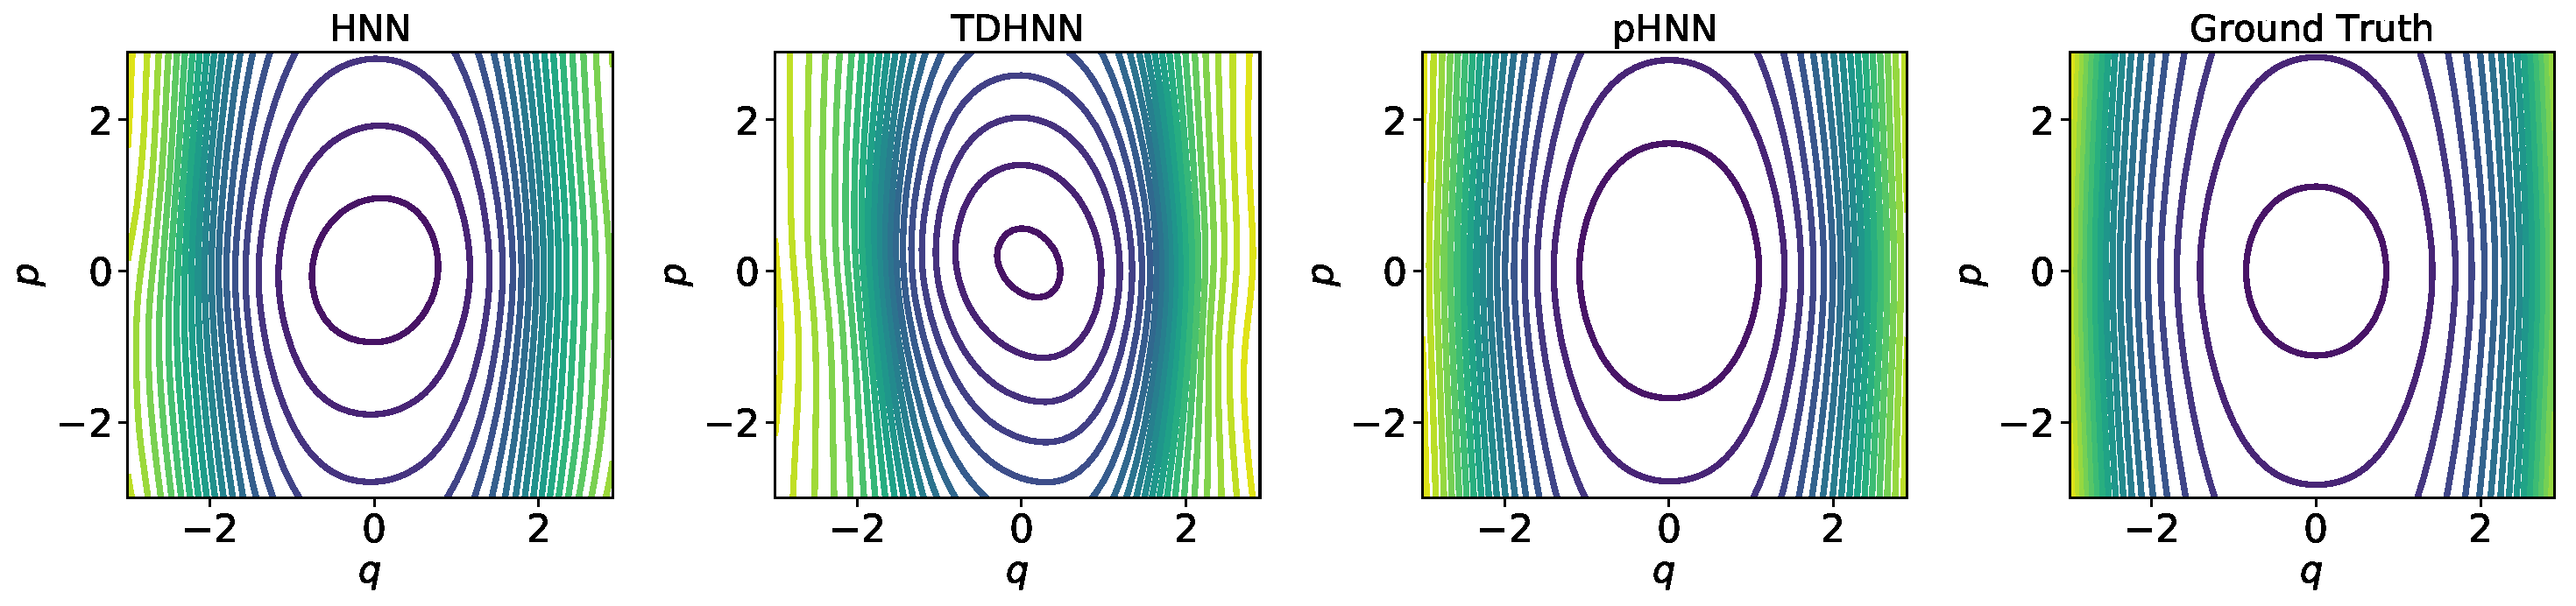
\includegraphics[width=\textwidth]{figures/figures/relativity/1/relativity_hamiltonian_0.pdf}
\caption{The learnt Hamiltonian across methods}
\end{subfigure}
\begin{subfigure}[b]{0.48\textwidth}
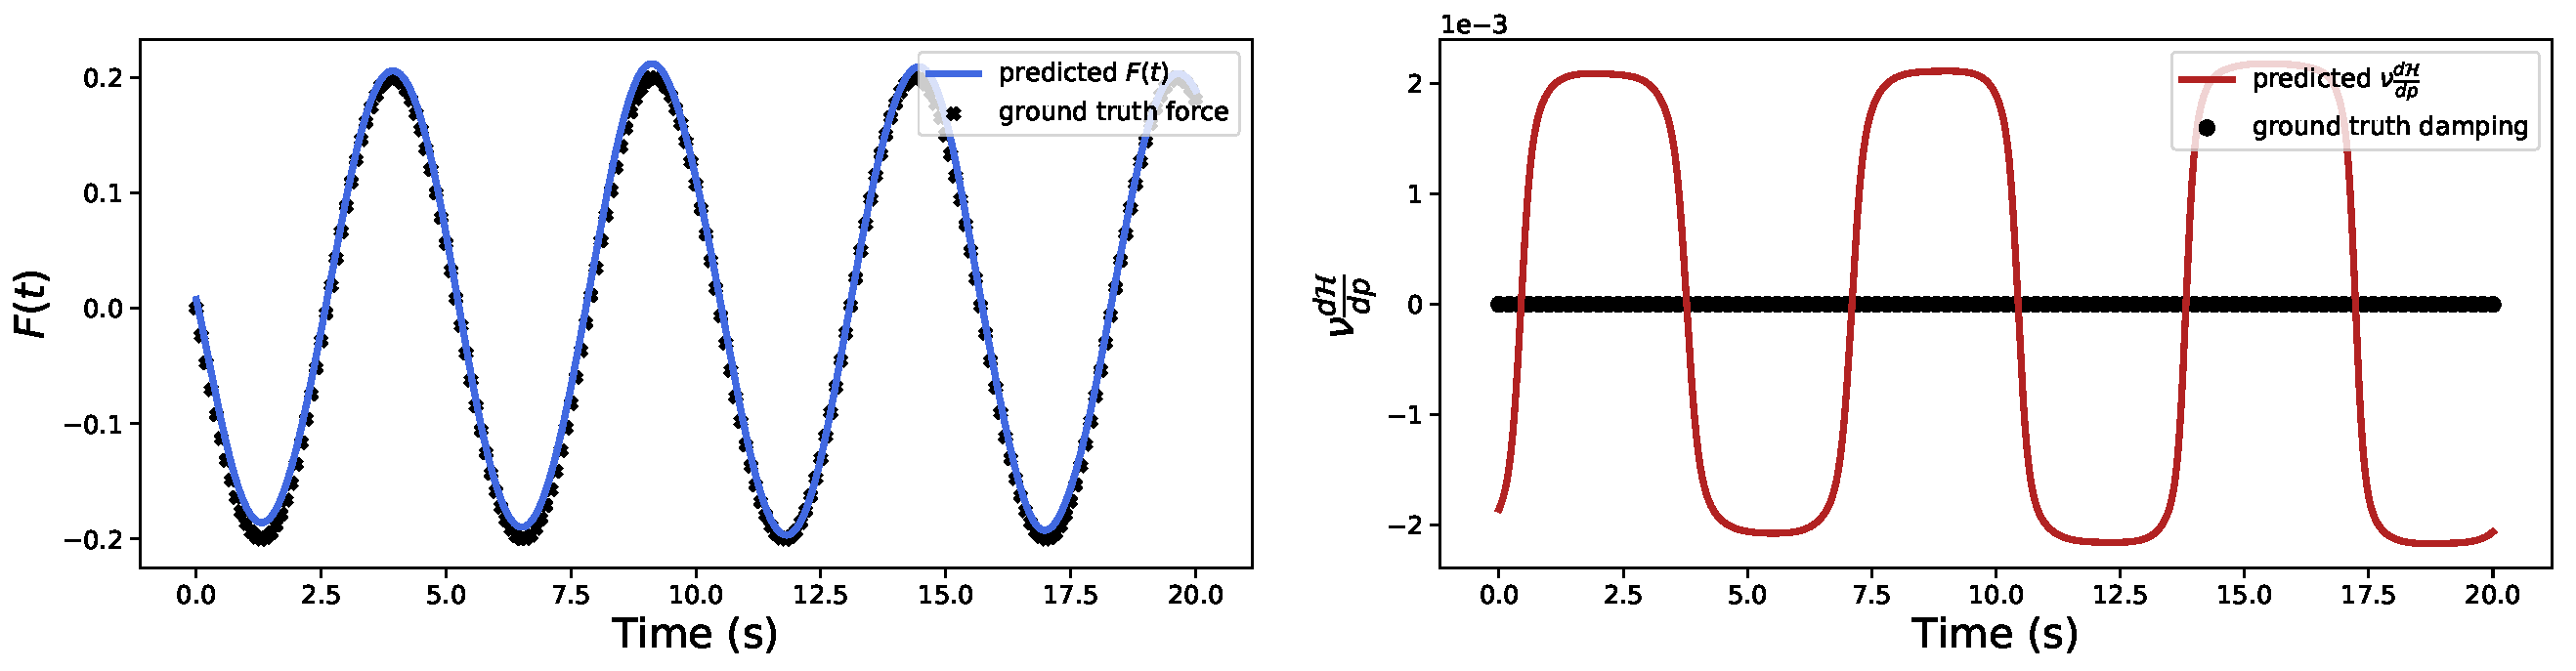
\includegraphics[width=\textwidth]{figures/figures/relativity/1/relativity_dpdt_new_0.pdf}
\caption{The learnt force and damping of TDHNN4}
\end{subfigure}
\label{duffing_1_full}
\end{figure}

\pagebreak
\onecolumn
\subsection*{C}
During the training of HNN, the authors add gaussian noise with a standard deviation $\sigma=0.1$ to the input state vector data. The reason this is done is to ensure the model is robustly trained. We run a set of experiments to test the robustness to this 'noisy' input. 
\begin{figure}[h!]
\centering
\captionsetup{justification=centering}
\begin{subfigure}[b]{0.42\textwidth}
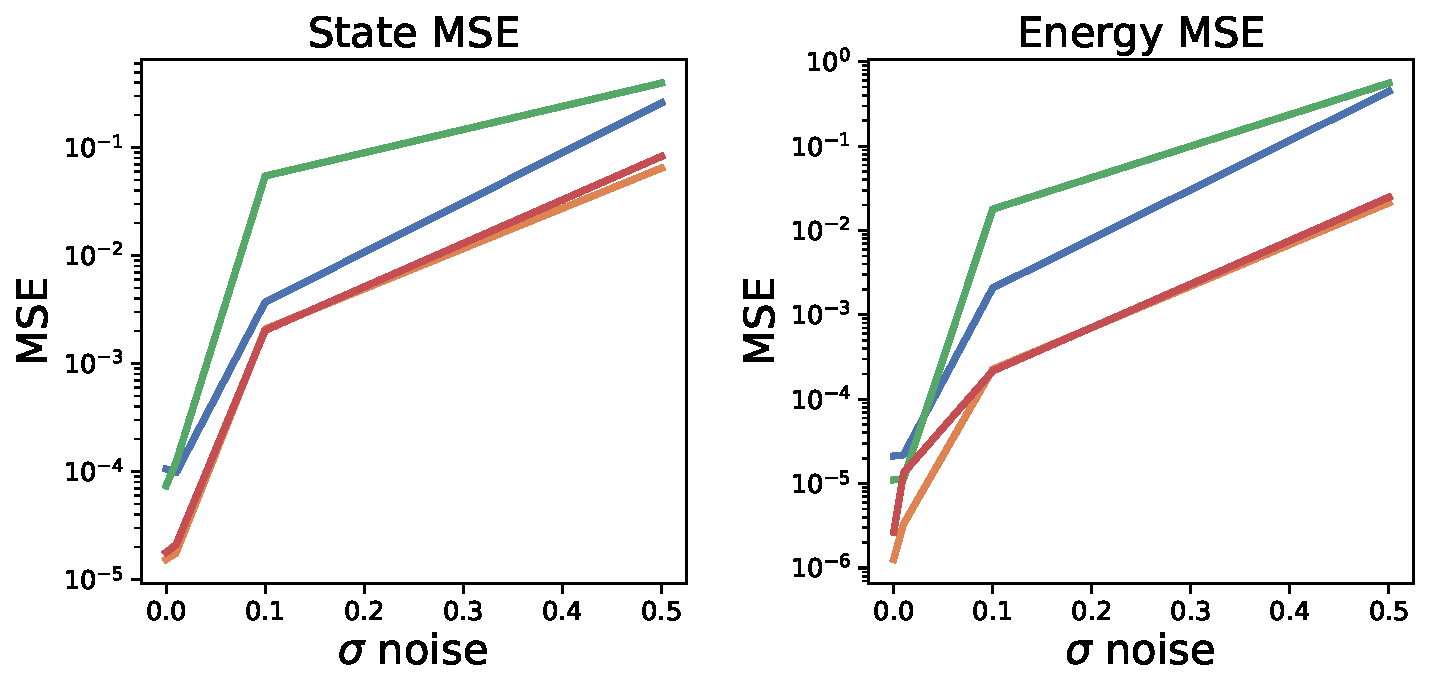
\includegraphics[width=\textwidth]{figures/figures/mass_spring/1/mass_spring_noise_scaling.pdf}
\caption{mass spring}
\end{subfigure}
\begin{subfigure}[b]{0.42\textwidth}
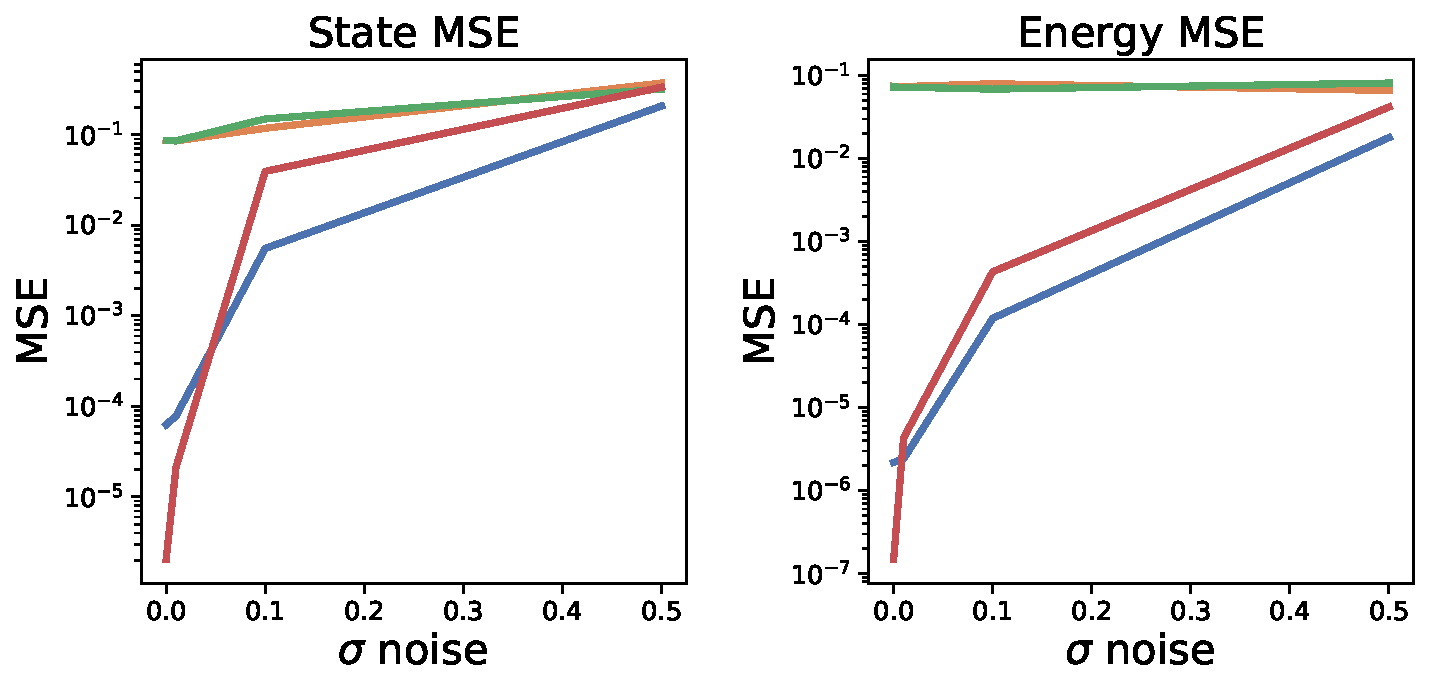
\includegraphics[width=\textwidth]{figures/figures/damped/1/damped_noise_scaling.pdf}
\caption{damped}
\end{subfigure}
\begin{subfigure}[b]{0.42\textwidth}
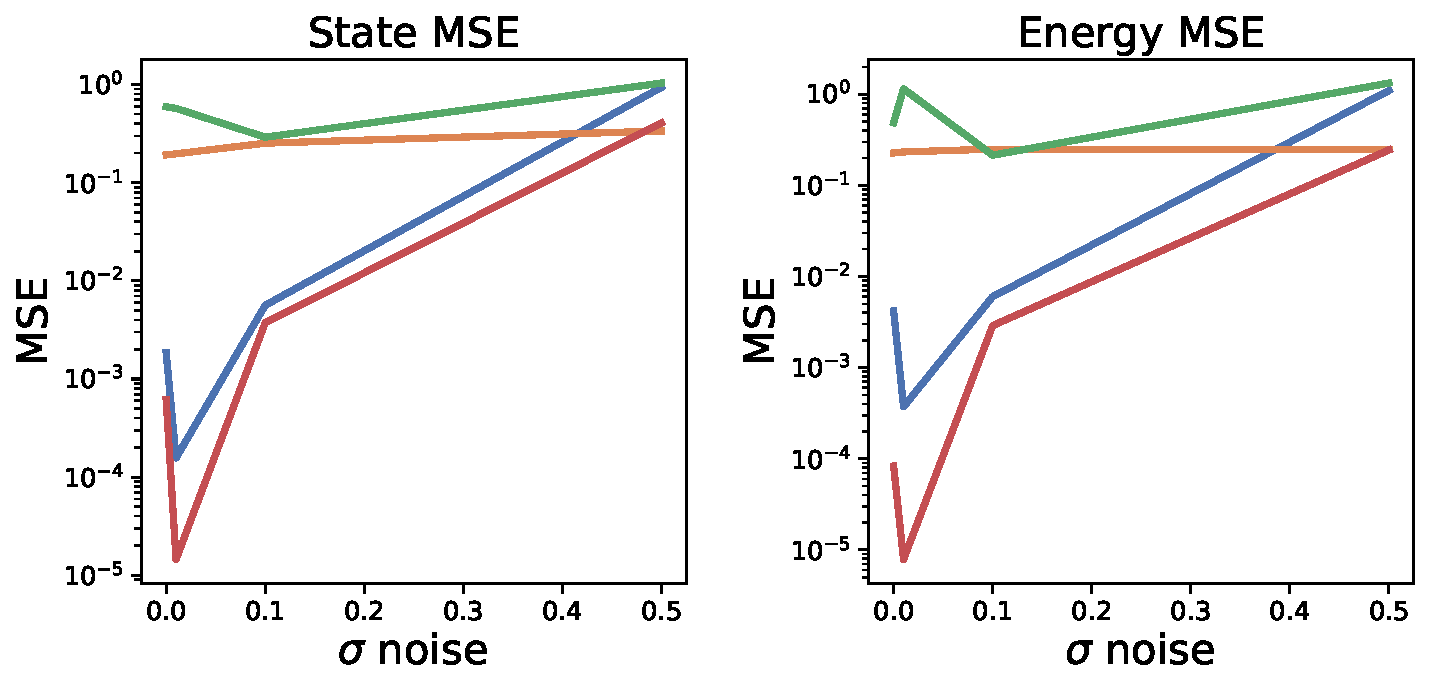
\includegraphics[width=\textwidth]{figures/figures/forced_mass_spring/1/forced_mass_spring_noise_scaling.pdf}
\caption{forced mass spring (I)}
\end{subfigure}
\begin{subfigure}[b]{0.42\textwidth}
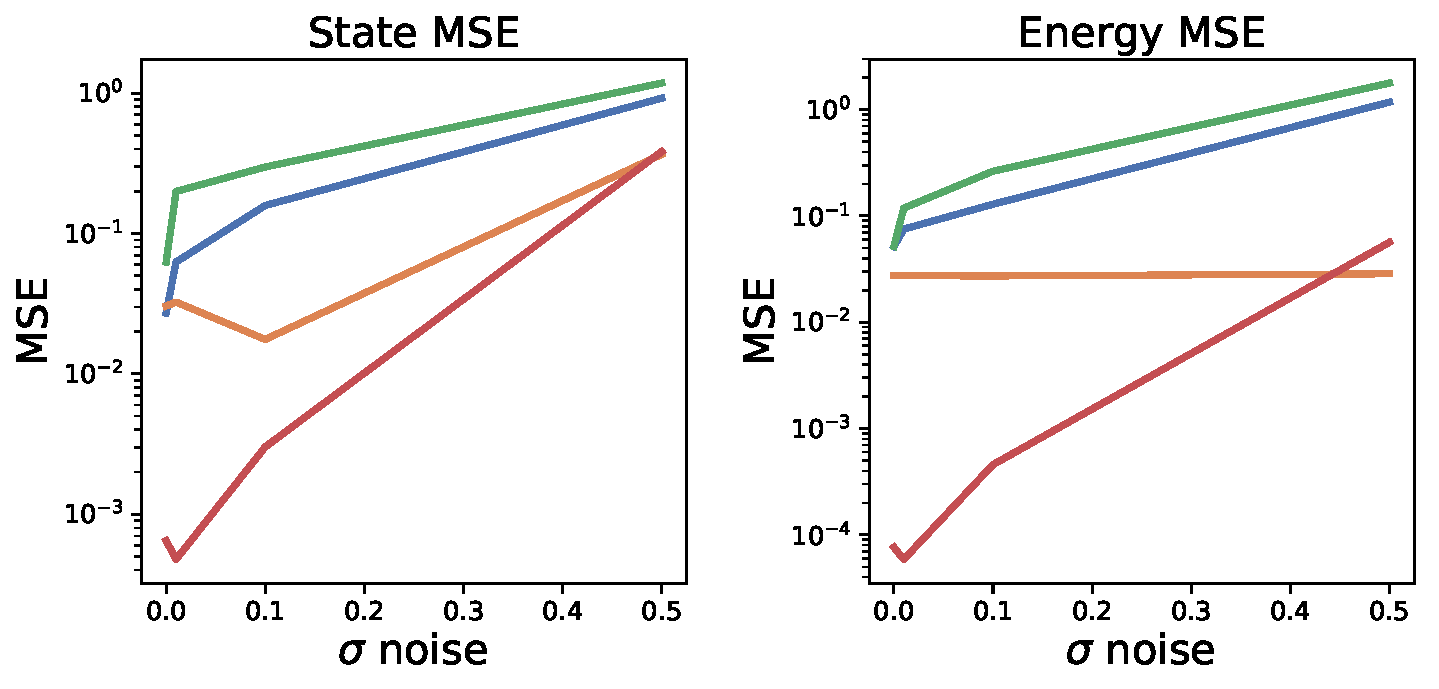
\includegraphics[width=\textwidth]{figures/figures/forced_mass_spring/2/forced_mass_spring_noise_scaling.pdf}
\caption{forced mass spring (II)}
\end{subfigure}
\begin{subfigure}[b]{0.42\textwidth}
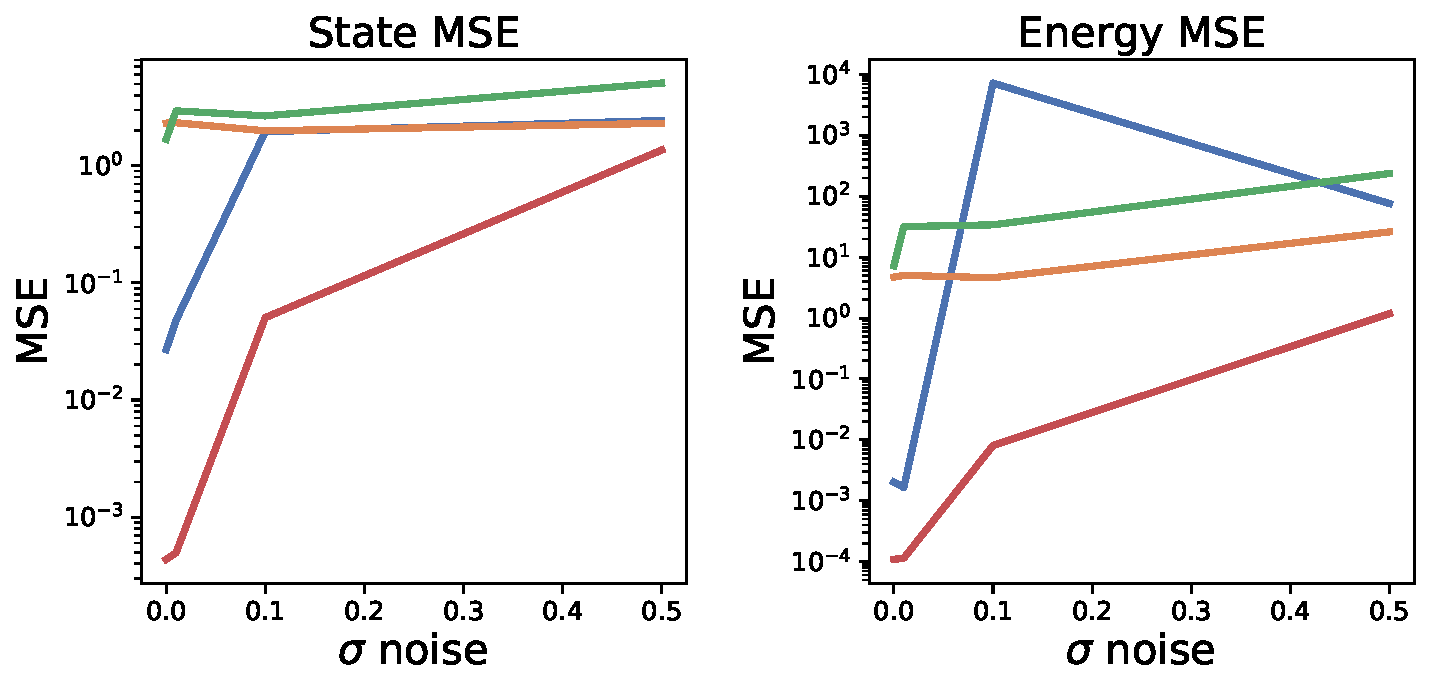
\includegraphics[width=\textwidth]{figures/figures/duffing/1/duffing_noise_scaling.pdf}
\caption{duffing}
\end{subfigure}
\begin{subfigure}[b]{0.42\textwidth}
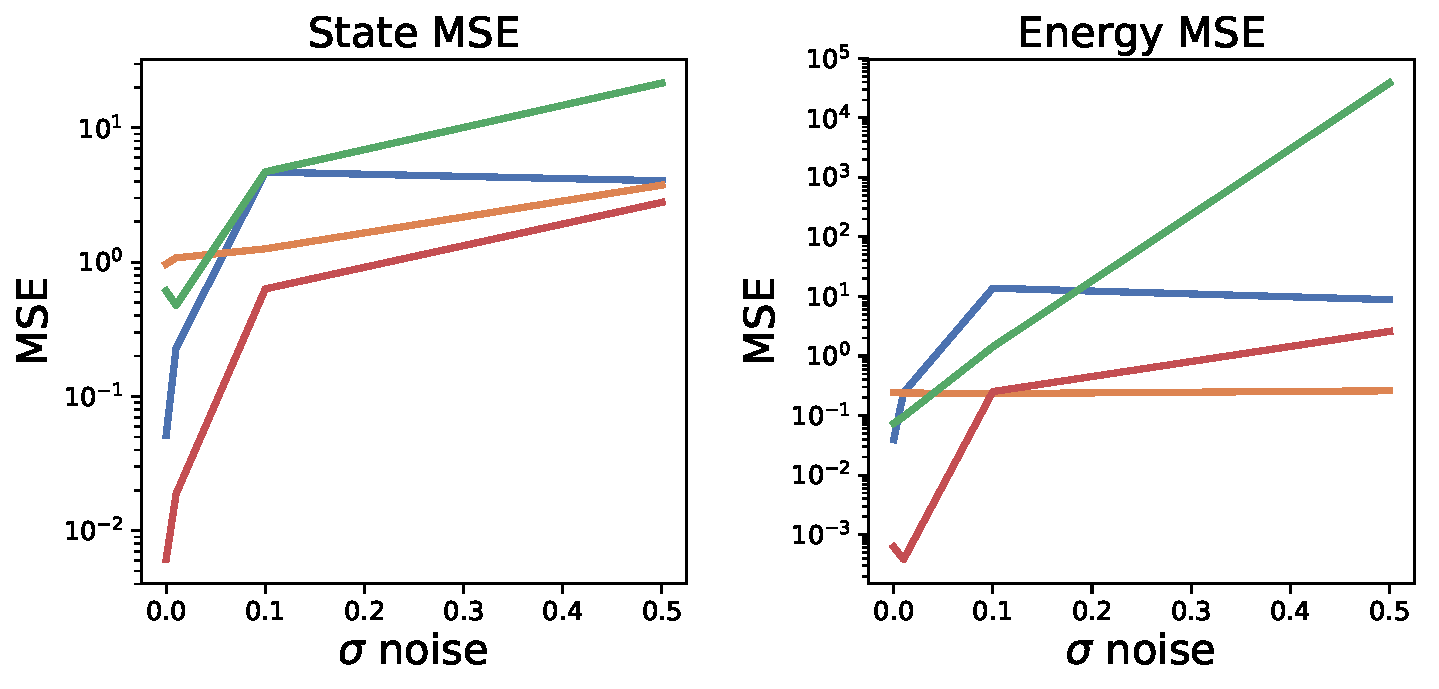
\includegraphics[width=\textwidth]{figures/figures/relativity/1/relativity_noise_scaling.pdf}
\caption{relativity}
\end{subfigure}
\end{figure}
\subsection*{D}
\begin{figure}[!htb]
\centering
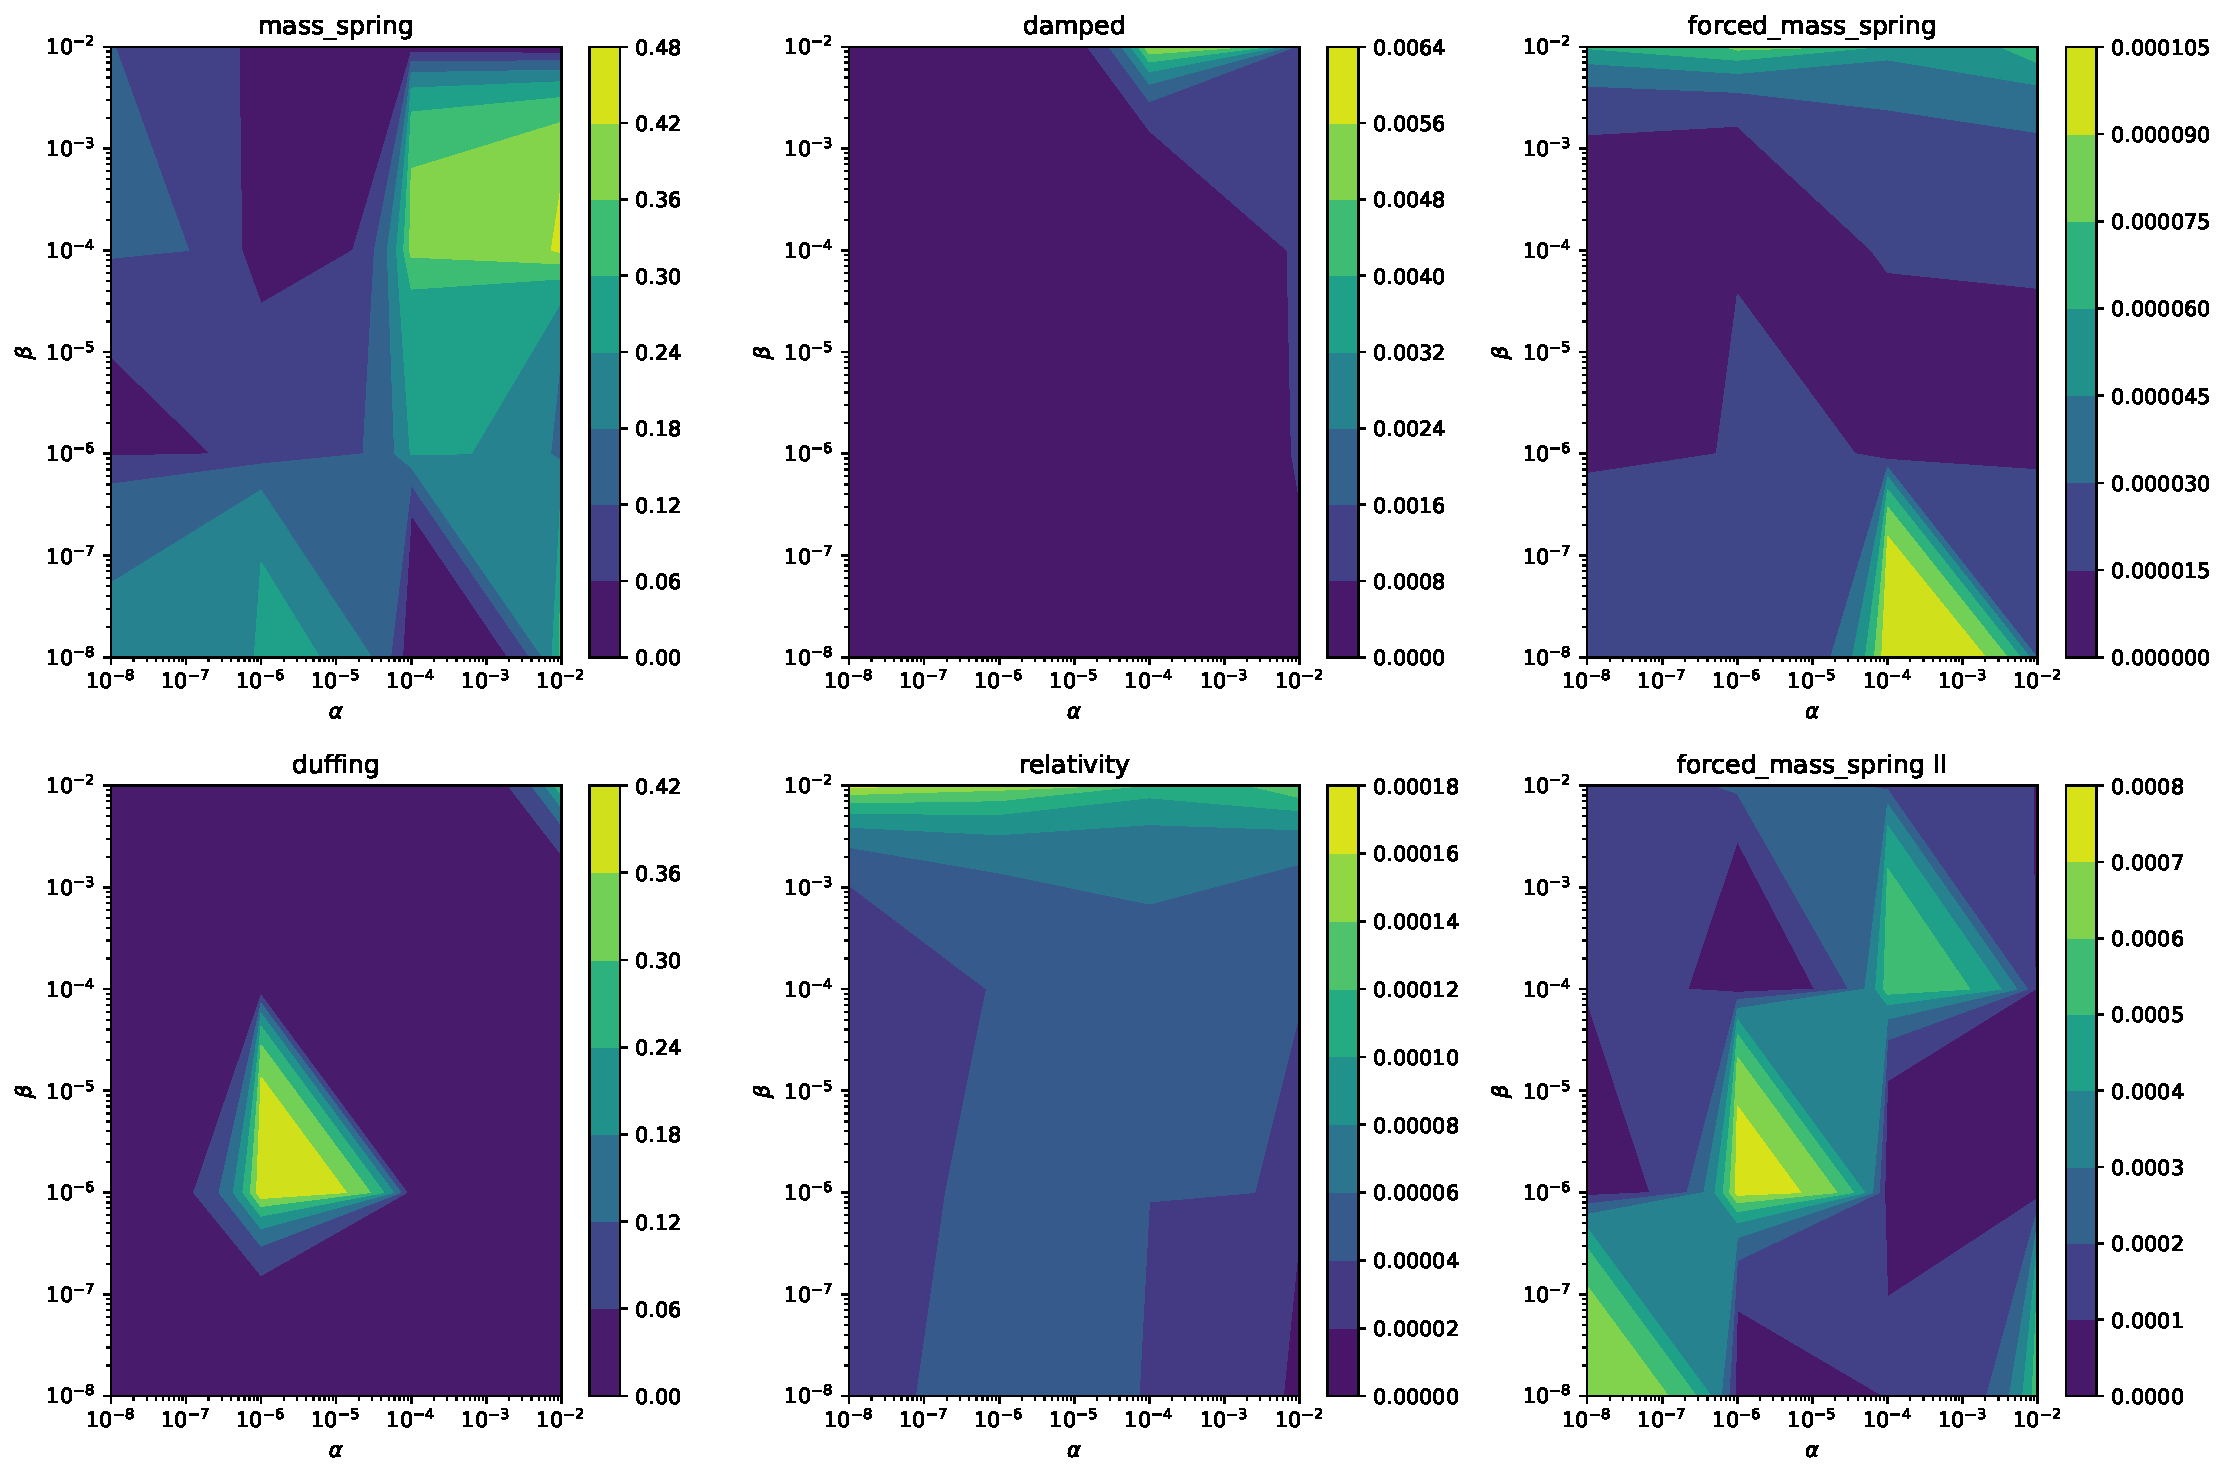
\includegraphics[width=.5\textwidth, height=5cm]{figures/forceanddampingregulariseroptimisation.pdf}
\caption{Hyperparameter Optimization for TDHNN4. We plot, for each system, the validation loss as a function of the $\alpha$ and $\beta$ parameters from the loss in eqn. 5}
\end{figure}

\end{document}